% !TeX program = xelatex
% !TeX encoding = UTF-8
% ==============================================================================
% KHUNG LÝ THUYẾT MÔ HÌNH
% Hệ ký hiệu thống nhất với "Bài báo chính.tex"; nhãn phương trình dùng lại
% cùng tên để hai văn bản đối chiếu chéo được.
% Hình trong thư mục hinh_ly_thuyet/ sinh từ chính chuỗi dữ liệu của pipeline.
% ==============================================================================
\documentclass[12pt,a4paper]{article}

\usepackage{fontspec}
\usepackage{unicode-math}
\IfFontExistsTF{Times New Roman}{\setmainfont{Times New Roman}}{\setmainfont{Liberation Serif}}
\IfFontExistsTF{Cambria Math}{\setmathfont{Cambria Math}}{\setmathfont{LibertinusMath-Regular.otf}}

\usepackage[a4paper,top=2.5cm,bottom=2.5cm,left=2.5cm,right=2.5cm]{geometry}
\usepackage{setspace}
\onehalfspacing
\usepackage{indentfirst}
\setlength{\parindent}{0.7cm}
\setlength{\parskip}{0.2em}
\emergencystretch=2em

\usepackage{microtype}
\usepackage{amsmath}
\usepackage{amsthm}
\usepackage{mathtools}
\numberwithin{equation}{section}

\usepackage{graphicx}
\usepackage{booktabs}
\usepackage{tabularx}
\usepackage{array}
\usepackage{longtable}
\usepackage{float}
\usepackage{enumitem}
\setlist[itemize]{leftmargin=1.5em,itemsep=0.15em,topsep=0.15em}
\setlist[enumerate]{leftmargin=1.8em,itemsep=0.15em,topsep=0.15em}

\usepackage{fancyhdr}
\pagestyle{fancy}
\fancyhf{}
\fancyhead[L]{\footnotesize\itshape Khung lý thuyết bài báo}
\fancyhead[R]{\footnotesize\thepage}
\renewcommand{\headrulewidth}{0.4pt}

\usepackage{caption}
\captionsetup{font=small,labelfont=bf}
\renewcommand{\tablename}{Bảng}
\renewcommand{\figurename}{Hình}
\renewcommand{\proofname}{Chứng minh}
\renewcommand{\abstractname}{Tóm tắt}

\newcolumntype{Y}{>{\raggedright\arraybackslash}X}
\newcolumntype{C}{>{\centering\arraybackslash}X}

\usepackage[dvipsnames,table]{xcolor}
\definecolor{NavyLink}{RGB}{0,68,148}      % Xanh dương đậm rõ ràng cho liên kết nội bộ
\definecolor{CiteLink}{RGB}{14,116,56}     % Xanh lá học thuật rõ nét cho trích dẫn
\definecolor{UrlLink}{RGB}{178,34,34}      % Đỏ gạch cho URL

\usepackage[unicode,colorlinks=true,linkcolor=NavyLink,citecolor=CiteLink,urlcolor=UrlLink]{hyperref}
\usepackage{cleveref}
\crefname{section}{Mục}{Các mục}
\Crefname{section}{Mục}{Các mục}
\crefname{subsection}{Mục}{Các mục}
\Crefname{subsection}{Mục}{Các mục}
\crefname{equation}{}{}
\Crefname{equation}{}{}
\crefname{table}{Bảng}{Các bảng}
\Crefname{table}{Bảng}{Các bảng}
\crefname{figure}{Hình}{Các hình}
\Crefname{figure}{Hình}{Các hình}
\crefname{assumption}{Giả định}{Các giả định}
\Crefname{assumption}{Giả định}{Các giả định}
\crefname{definition}{Định nghĩa}{Các định nghĩa}
\Crefname{definition}{Định nghĩa}{Các định nghĩa}

\theoremstyle{definition}
\newtheorem{definition}{Định nghĩa}[section]
\newtheorem{assumption}{Giả định}[section]
\newtheorem{proposition}{Mệnh đề}[section]
\newtheorem{remark}{Nhận xét}[section]

% --- Ký hiệu: đồng bộ với "Bài báo chính.tex" -------------------------------
\newcommand{\R}{\mathbb{R}}
\newcommand{\E}{\mathbb{E}}
\newcommand{\Var}{\operatorname{Var}}
\newcommand{\Cov}{\operatorname{Cov}}
\newcommand{\Prob}{\mathbb{P}}
\newcommand{\diag}{\operatorname{diag}}
\newcommand{\softplus}{\operatorname{softplus}}
\newcommand{\sigmoid}{\operatorname{sigmoid}}
\newcommand{\KL}{\operatorname{KL}}
\newcommand{\ELBO}{\operatorname{ELBO}}
\newcommand{\AIC}{\operatorname{AIC}}
\newcommand{\BIC}{\operatorname{BIC}}
\newcommand{\MAE}{\operatorname{MAE}}
\newcommand{\RMSE}{\operatorname{RMSE}}
\newcommand{\QLIKE}{\operatorname{QLIKE}}
\newcommand{\NLS}{\operatorname{NLS}}
\newcommand{\VaR}{\operatorname{VaR}}
\newcommand{\Data}{\mathcal{D}}
\newcommand{\Info}{\mathcal{F}}
\newcommand{\Param}{\symbf{\theta}}
\newcommand{\Xvec}{\symbf{X}}
\newcommand{\Pmat}{\symbf{P}}
\newcommand{\bmgamma}{\symbf{\gamma}}
\newcommand{\vecphi}{\symbf{\phi}}
\newcommand{\vech}{\operatorname{vech}}
\newcommand{\diff}{\mathrm{d}}

\title{\Large \textbf{KHUNG SƯỜN LÝ THUYẾT NGHIÊN CỨU KHOA HỌC} Mô hình MS-GARCH-X với phân phối sai số Student-t cho hợp đồng tương lai VN30F1M\\
}
\author{Nguyễn Hoài Nam, Nguyễn Thuận Hiếu, Đặng Chí Hiếu}
\date{\normalsize Tháng 9 năm 2026}

\begin{document}
	\maketitle
	\thispagestyle{empty}
	\newpage
	% ==============================================================================
	\section*{Bảng ký hiệu}
	\addcontentsline{toc}{section}{Bảng ký hiệu}
	% ==============================================================================
	
	{\footnotesize
		\begin{longtable}{@{}p{3.0cm}>{\raggedright\arraybackslash}p{12.2cm}@{}}
			\toprule
			\textbf{Ký hiệu} & \textbf{Ý nghĩa} \\
			\midrule
			\endfirsthead
			\toprule
			\textbf{Ký hiệu} & \textbf{Ý nghĩa} \\
			\midrule
			\endhead
			\bottomrule
			\endfoot
			$r_t$ & Lợi suất logarit theo phần trăm tại phiên $t$. \\
			$\varepsilon_t$ & Nhiễu của phương trình trung bình. \\
			$z_t$ & Sai số chuẩn hóa, $\E[z_t]=0$ và $\Var(z_t)=1$. \\
			$h_{t,s}$ & Phương sai có điều kiện tại $t$ khi $S_t=s$. \\
			$\bar\mu_{t-1},\ \bar h_{t-1}$ & Trung bình và phương sai hỗn hợp thu gọn tại $t-1$. \\
			$\bar\varepsilon_{t-1}$ & Phần dư thu gọn, $\bar\varepsilon_{t-1}=r_{t-1}-\bar\mu_{t-1}$. \\
			$S_t$ & Trạng thái ẩn, $S_t\in\{1,2\}$. \\
			$p_{ij}$ & Xác suất chuyển từ trạng thái $i$ sang $j$. \\
			$\Pmat$ & Ma trận chuyển trạng thái Markov. \\
			$\xi_{t\mid u}(s)$ & Xác suất $S_t=s$ có điều kiện trên thông tin đến $u$. \\
			$\pi_s,\ d_s$ & Xác suất dừng và thời gian tồn tại kỳ vọng của trạng thái $s$. \\
			$\mu_s,\omega_s,\alpha_s,\beta_s$ & Hệ số trung bình và phương sai của trạng thái $s$. \\
			$\bmgamma_s$ & Vector hệ số biến ngoại sinh của trạng thái $s$. \\
			$\theta_s$ & Hệ số đòn bẩy (hiệu ứng dấu) của trạng thái $s$ trong đặc tả EGARCH. \\
			$\Xvec_{t-1}$ & Vector $k$ biến ngoại sinh, biết trước thời điểm dự báo. \\
			$\nu$ & Bậc tự do của phân phối Student-t chuẩn hóa. \\
			$t^{*}_{\nu}$ & Phân phối Student-t chuẩn hóa về phương sai đơn vị. \\
			$\Param$ & Vector toàn bộ tham số liên tục của mô hình. \\
			$\vecphi$ & Ảnh của $\Param$ trên không gian không ràng buộc $\R^{d}$. \\
			$\Info_{t-1}$ & Tập thông tin đến cuối phiên $t-1$. \\
			$\Data_T$ & Toàn bộ dữ liệu dùng cho suy diễn đến $T$. \\
			$\mathcal{L}(\Param;\Data_T)$ & Hàm likelihood của mẫu huấn luyện. \\
			$\ell_T(\Param)$ & Hàm log-likelihood, $\ell_T=\ln\mathcal{L}$. \\
			$p(\Param),\ p(\Param\mid\Data_T)$ & Mật độ tiên nghiệm và hậu nghiệm. \\
			$q(\vecphi)$ & Phân phối xấp xỉ hậu nghiệm trong suy diễn biến phân. \\
			$\diag(\cdot)$ & Ma trận đường chéo tạo từ các phần tử trong ngoặc. \\
			$\vech(\cdot)$ & Vector hóa phần tam giác dưới của một ma trận. \\
			$RV_t$ & Biến động thực tế, đo trên thang phương sai. \\
			$\VaR_{t,\alpha}$ & Giá trị chịu rủi ro tại mức xác suất đuôi $\alpha$. \\
		\end{longtable}
	}
	
	\newpage
	% 
	
	% ==============================================================================
	\section{Dữ liệu}\label{sec:data}
	% ==============================================================================
	
	\subsection{Nguồn dữ liệu và xây dựng chuỗi}\label{subsec:data-source}
	Dữ liệu là chuỗi giá trong ngày của hợp đồng tương lai chỉ số VN30 kỳ hạn gần nhất
	(VN30F1M), giai đoạn từ ngày $07/11/2017$ đến ngày $17/07/2026$. Chuỗi lợi suất logarit
	theo phần trăm được xác định bởi
	\begin{equation}
		r_t = 100\times\ln\!\left(P_t/P_{t-1}\right),
		\label{eq:return}
	\end{equation}
	trong đó $P_t$ là giá đóng cửa phiên $t$. Sau khi làm sạch và loại phiên đầu tiên (không
	xác định được lợi suất), mẫu gồm $2170$ quan sát ngày.
	
	Đại lượng đại diện cho biến động thực tế được xây dựng từ lợi suất trong ngày:
	\begin{equation}
		RV_t=\sum_{m=1}^{M_t} r_{t,m}^{2}
		\label{eq:realized-variance}
	\end{equation}
	với $r_{t,m}$ là lợi suất logarit của thanh giá thứ $m$ trong phiên $t$ và $M_t$ là số
	thanh giá của phiên đó. Vì \eqref{eq:realized-variance} là tổng bình phương, $RV_t$ nằm
	trên \emph{thang phương sai}, cùng đơn vị với $h_{t,s}$; sự thống nhất đơn vị này là điều
	kiện để các hàm tổn thất ở \cref{sec:oos} có nghĩa.
	
	Vector biến ngoại sinh gồm $k=2$ thành phần, đều trễ một bậc để bảo đảm khả dụng tại thời
	điểm lập dự báo:
	\begin{equation}
		\Xvec_{t-1}=\left(\ \ln\!\left(1+V_{t-1}\right),\ \ \ln\!\left(RV_{t-1}+\epsilon\right)\ \right)^{\!\top},
		\label{eq:exog}
	\end{equation}
	với $V_{t-1}$ là khối lượng giao dịch và $\epsilon>0$ là hằng số nhỏ tránh logarit của
	không. Phép biến đổi logarit làm giảm độ lệch phải rất mạnh của hai đại lượng gốc. Cả hai
	thành phần được chuẩn hóa z-score bằng trung bình và độ lệch chuẩn \emph{của riêng tập
		huấn luyện}; dùng thống kê toàn mẫu sẽ đưa thông tin của giai đoạn kiểm định vào giai
	đoạn huấn luyện và làm mọi kết quả ngoài mẫu mất hiệu lực.
	\subsection{Thống kê mô tả}\label{subsec:descriptive}
	
	\begin{table}[H]
		\centering\footnotesize
		\setlength{\tabcolsep}{5pt}
		\caption{Thống kê mô tả của lợi suất, biến động thực tế và biến ngoại sinh}
		\label{tab:descriptive}
	\begin{tabularx}{\textwidth}{l C C C C C C C}
		\toprule
		\textbf{Chuỗi} & \textbf{Số quan sát} & \textbf{Trung bình} & \textbf{Độ lệch chuẩn} & \textbf{Skewness} & \textbf{Kurtosis} & \textbf{Giá trị nhỏ nhất} & \textbf{Giá trị lớn nhất} \\
		\midrule
		$r_t$ & 2170 & 0{,}0381 & 1{,}5070 & $-0{,}829$ & 9{,}026 & $-11{,}6612$ & 6{,}7631 \\
		\addlinespace[0.2em]
		$RV_t$ & 2170 & 1{,}3275 & 2{,}3474 & 7{,}195 & 86{,}957 & 0{,}0304 & 43{,}2472 \\
		\addlinespace[0.2em]
		$X_1$: Khối lượng & 2170 & 0{,}1285 & 0{,}9500 & $-1{,}444$ & 5{,}764 & $-4{,}0025$ & 2{,}0458 \\
		$X_2$: $RV$ trễ & 2170 & $-0{,}0170$ & 0{,}9666 & 0{,}484 & 3{,}180 & $-2{,}9491$ & 3{,}8108 \\
		\bottomrule
	\end{tabularx}
		\raggedright\footnotesize
		\textit{Ghi chú:} Lợi suất tính theo phần trăm. Độ lệch chuẩn dùng ước lượng mẫu với bậc
		tự do $n-1$; skewness và kurtosis chuẩn hóa theo cùng độ lệch chuẩn đó. Hai biến
		ngoại sinh đã chuẩn hóa z-score theo thống kê tập huấn luyện, nên trung bình của chúng
		trên toàn mẫu không bằng đúng không.
	\end{table}
	
	\begin{figure}[H]
		\centering
		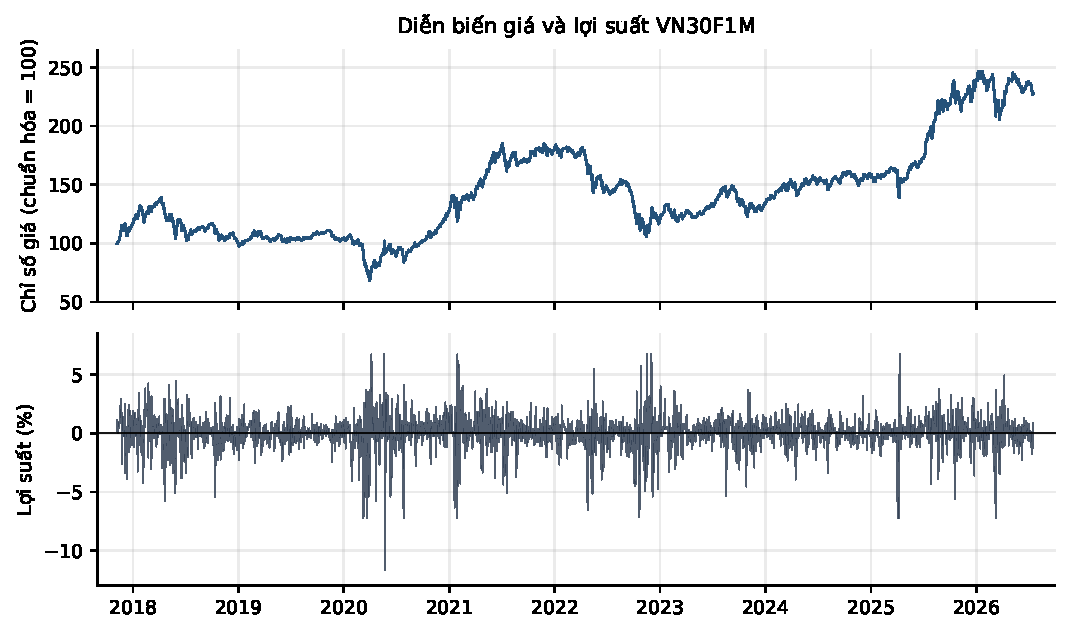
\includegraphics[width=\textwidth]{hinh_ly_thuyet/fig_gia_loi_suat.pdf}
		\caption{Diễn biến giá đóng cửa và chuỗi lợi suất logarit VN30F1M giai đoạn 2017--2026 trên toàn bộ mẫu dữ liệu (2170 quan sát ngày).}
		\label{fig:gia-loi-suat}
	\end{figure}
	
	\begin{figure}[H]
		\centering
		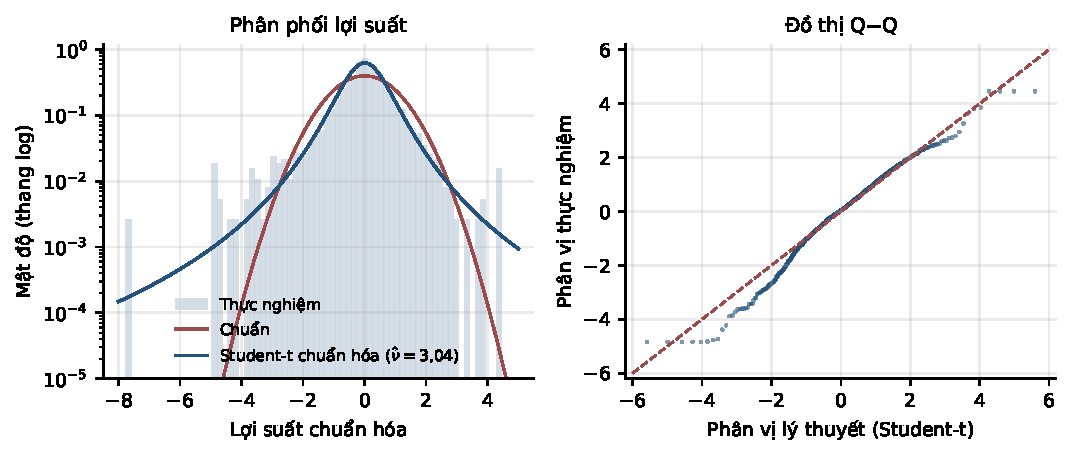
\includegraphics[width=\textwidth]{hinh_ly_thuyet/fig_phan_phoi.pdf}
		\caption{Phân phối lợi suất chuẩn hóa (thang logarit) và đồ thị Q--Q so với Student-t
			chuẩn hóa.}
		\label{fig:phan-phoi}
	\end{figure}
	
	\begin{figure}[H]
		\centering
		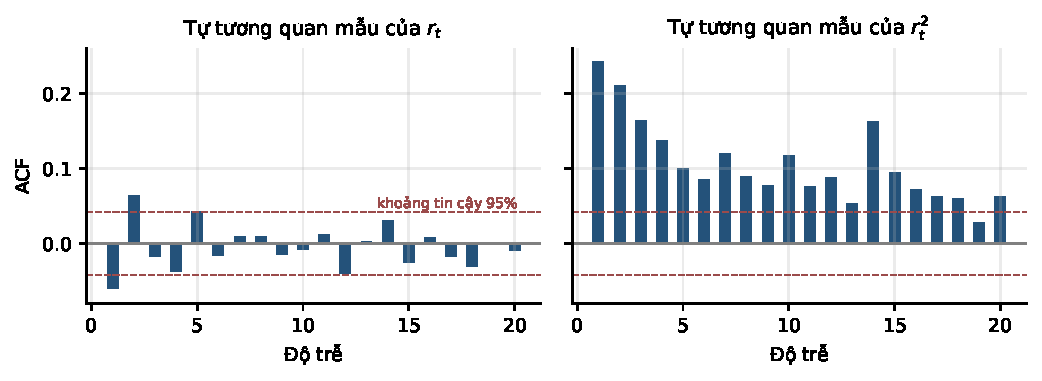
\includegraphics[width=\textwidth]{hinh_ly_thuyet/fig_acf.pdf}
		\caption{Tự tương quan mẫu của $r_t$ và $r_t^{2}$, kèm khoảng tin cậy $95\%$.}
		\label{fig:acf}
	\end{figure}
	
	\begin{figure}[H]
		\centering
		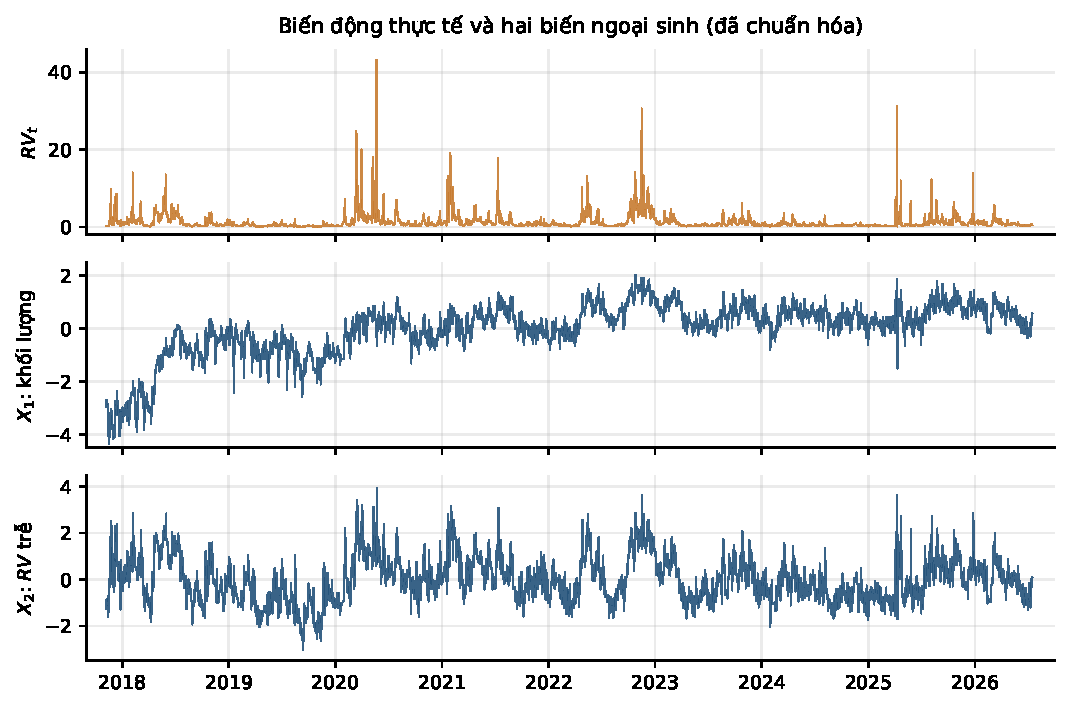
\includegraphics[width=\textwidth]{hinh_ly_thuyet/fig_rv_exog.pdf}
		\caption{Biến động thực tế $RV_t$ và hai biến ngoại sinh sau chuẩn hóa.}
		\label{fig:rv-exog}
	\end{figure}
	
	% ==============================================================================
	\section{Đặc tả mô hình}\label{sec:models}
	% ==============================================================================
	
	\subsection{Phân phối sai số}\label{subsec:errors}
	Mọi mô hình viết dưới dạng $r_t=\mu_{(\cdot)}+\varepsilon_t$ với
	$\varepsilon_t=\sqrt{h_{t,(\cdot)}}\,z_t$ và $z_t$ độc lập cùng phân phối, chuẩn hóa sao
	cho $\E[z_t]=0$, $\Var(z_t)=1$. Hai hàm mật độ phân phối xác suất chuẩn hóa:
	\begin{align}
		f_{\mathcal{N}}(z) &= \frac{1}{\sqrt{2\pi}}\exp\!\left(-\tfrac{1}{2}z^{2}\right),
		\label{eq:normal-density}\\[0.2em]
		f_{t^{*}}(z;\nu) &= \frac{\Gamma\!\left(\frac{\nu+1}{2}\right)}
		{\sqrt{\pi(\nu-2)}\,\Gamma\!\left(\frac{\nu}{2}\right)}
		\left(1+\frac{z^{2}}{\nu-2}\right)^{-\frac{\nu+1}{2}},\qquad \nu>2.
		\label{eq:std-t-density}
	\end{align}
	Mật độ \eqref{eq:std-t-density} là phân phối Student-t đã chuẩn hóa về phương sai đơn vị,
	ký hiệu $t^{*}_{\nu}$. Thừa số $\nu-2$ thay cho $\nu$ dưới dấu căn chính là phép co giãn
	bảo đảm $\Var(z_t)=1$; nhờ đó $h_{t,s}$ giữ đúng ý nghĩa phương sai có điều kiện và so
	sánh trực tiếp được với trường hợp sai số chuẩn. Ràng buộc $\nu>2$ vì vậy không phải quy
	ước kỹ thuật mà là điều kiện tồn tại của chính phép chuẩn hóa.
	
	\subsection{Họ mô hình một trạng thái}\label{subsec:single-regime}
	Ba mô hình đối chứng là các trường hợp riêng của một đặc tả chung:
	\begin{equation}
		r_t=\mu+\varepsilon_t,\qquad
		h_t=\omega+\alpha\varepsilon_{t-1}^{2}+\beta h_{t-1}+\bmgamma^{\top}\Xvec_{t-1}.
		\label{eq:garchx}
	\end{equation}
	Trong \eqref{eq:garchx}, $\omega$ là mức phương sai nền, $\alpha$ đo phản ứng của phương
	sai với cú sốc mới, $\beta$ đo mức độ dai dẳng của biến động, và $\bmgamma$ đo ảnh hưởng
	của thông tin ngoại sinh.
	
	\begin{table}[H]
		\centering\footnotesize
		\setlength{\tabcolsep}{4pt}
		\caption{Sáu mô hình một trạng thái: hai họ phương sai $\times$ ba mức cấu trúc}
		\label{tab:single-models}
		\begin{tabularx}{\textwidth}{l c c c c Y}
			\toprule
			\textbf{Mô hình} & \textbf{Phương trình} & \textbf{Phân phối $z_t$} & \textbf{$\bmgamma$} & \textbf{Số tham số} & \textbf{Thành phần cấu trúc} \\
			\midrule
			GARCH chuẩn & \eqref{eq:garchx} & $\mathcal{N}(0,1)$ & $\equiv\symbf 0$ & $4$ & Mốc so sánh \\
			GARCH Student-$t$ & \eqref{eq:garchx} & $t^{*}_{\nu}$ & $\equiv\symbf 0$ & $5$ & Đuôi dày \\
			GARCH-X Student-$t$ & \eqref{eq:garchx} & $t^{*}_{\nu}$ & $\in\R^{k}$ & $5+k$ & Đuôi dày, ngoại sinh \\
			\addlinespace[0.3em]
			EGARCH chuẩn & \eqref{eq:egarchx} & $\mathcal{N}(0,1)$ & $\equiv\symbf 0$ & $5$ & Bất đối xứng \\
			EGARCH Student-$t$ & \eqref{eq:egarchx} & $t^{*}_{\nu}$ & $\equiv\symbf 0$ & $6$ & Bất đối xứng, đuôi dày \\
			EGARCH-X Student-$t$ & \eqref{eq:egarchx} & $t^{*}_{\nu}$ & $\in\R^{k}$ & $6+k$ & Cả ba thành phần \\
			\bottomrule
		\end{tabularx}
		\vspace{0.3em}
		\raggedright\scriptsize
		\emph{Ghi chú:} Với $k=2$ biến ngoại sinh, GARCH-X Student-$t$ có $7$ tham số và
		EGARCH-X Student-$t$ có $8$. Chênh lệch cố định $+1$ giữa hai họ là hệ số đòn bẩy
		$\theta$ trong \eqref{eq:egarchx}.
	\end{table}

	\begin{assumption}[Điều kiện chính quy của mô hình một trạng thái]\label{as:single}
		$\omega>0$, $\alpha\ge 0$, $\beta\ge 0$. Dừng hiệp phương sai yếu khi $\alpha+\beta<1$,
		khi đó phương sai vô điều kiện là
		\begin{equation}
			\bar h=\frac{\omega}{1-\alpha-\beta}.
			\label{eq:garch-unconditional-var}
		\end{equation}
		Với sai số $t^{*}_{\nu}$, moment bậc bốn tồn tại khi $\nu>4$ và
		$3\alpha^{2}\frac{\nu-2}{\nu-4}+2\alpha\beta+\beta^{2}<1$.
	\end{assumption}
	
	\begin{remark}[Tính dương của phương sai khi có biến ngoại sinh]\label{rem:positivity}
		Trong \eqref{eq:garchx}, tổ hợp $\bmgamma^{\top}\Xvec_{t-1}$ có thể nhận giá trị âm, nên
		ràng buộc dấu của $(\omega,\alpha,\beta)$ \emph{không còn đủ} để bảo đảm $h_t>0$. Đây là
		khác biệt bản chất giữa GARCH-X và GARCH cổ điển. Tính dương phải được xử lý bằng một cơ
		chế tường minh, hoặc bằng ràng buộc miền giá trị, hoặc bằng hàm liên kết bảo toàn dấu.
		Trong nghiên cứu này, tính dương được kiểm tra hậu nghiệm: Tại nghiệm ước lượng của mọi
		mô hình, vế phải của \eqref{eq:garchx} dương tại mọi thời điểm trong mẫu, nên đặc tả cộng
		tính giữ nguyên hiệu lực.
	\end{remark}

	\subsection{Họ mô hình EGARCH}\label{subsec:egarch}
	Đặc tả \eqref{eq:garchx} cộng tính \emph{trên thang phương sai} và đối xứng: cú sốc
	$\varepsilon_{t-1}$ chỉ đi vào qua bình phương $\varepsilon_{t-1}^{2}$, nên một cú sốc âm
	và một cú sốc dương cùng độ lớn tác động hệt như nhau lên $h_t$. Họ EGARCH
	\cite{nelson1991} thay cả hai đặc điểm đó bằng cách mô hình hóa \emph{logarit} của phương
	sai:
	\begin{equation}
		\ln h_t=\omega+\alpha\left(\lvert z_{t-1}\rvert-\E\lvert z_{t-1}\rvert\right)
		+\theta\,z_{t-1}+\beta\ln h_{t-1}+\bmgamma^{\top}\Xvec_{t-1},
		\qquad z_{t-1}=\frac{\varepsilon_{t-1}}{\sqrt{h_{t-1}}}.
		\label{eq:egarchx}
	\end{equation}
	Bốn số hạng mang bốn vai trò tách bạch. Số hạng $\alpha(\lvert z_{t-1}\rvert-\E\lvert
	z_{t-1}\rvert)$ là \emph{hiệu ứng độ lớn}: nó phản ứng với biên độ cú sốc chuẩn hóa, đã
	trừ đi kỳ vọng nên có trung bình không. Số hạng $\theta z_{t-1}$ là \emph{hiệu ứng dấu},
	tức hiệu ứng đòn bẩy: khi $\theta<0$, một cú sốc âm làm tăng $\ln h_t$ nhiều hơn một cú
	sốc dương cùng độ lớn. Hệ số $\beta$ đo độ dai dẳng của log-phương sai, và
	$\bmgamma^{\top}\Xvec_{t-1}$ vẫn là kênh thông tin ngoại sinh như ở \eqref{eq:garchx}.

	Hằng số $\E\lvert z_t\rvert$ phụ thuộc phân phối sai số và có dạng đóng ở cả hai trường
	hợp dùng trong nghiên cứu:
	\begin{align}
		\E\lvert z_t\rvert &= \sqrt{\tfrac{2}{\pi}}
		&&\text{khi } z_t\sim\mathcal{N}(0,1),
		\label{eq:eabsz-normal}\\[0.2em]
		\E\lvert z_t\rvert &= \frac{2\sqrt{\nu-2}\;\Gamma\!\left(\frac{\nu+1}{2}\right)}
		{(\nu-1)\sqrt{\pi}\;\Gamma\!\left(\frac{\nu}{2}\right)}
		&&\text{khi } z_t\sim t^{*}_{\nu},\ \nu>2.
		\label{eq:eabsz-t}
	\end{align}
	Hai biểu thức này nhất quán với nhau: khi $\nu\to\infty$, tỷ số
	$\Gamma(\frac{\nu+1}{2})/\Gamma(\frac{\nu}{2})$ tiệm cận $\sqrt{\nu/2}$, nên vế phải của
	\eqref{eq:eabsz-t} hội tụ về $\sqrt{2/\pi}$ --- đúng bằng \eqref{eq:eabsz-normal}. Đây là
	một phép kiểm tra bắt buộc khi cài đặt, vì sai sót ở hằng số này làm lệch toàn bộ mức nền
	của phương trình phương sai mà không sinh ra bất kỳ cảnh báo số học nào.

	\begin{assumption}[Điều kiện chính quy của EGARCH]\label{as:egarch}
		Điều kiện dừng của lý thuyết là $\lvert\beta\rvert<1$; các hệ số $\omega$, $\alpha$,
		$\theta$ và $\bmgamma$ \emph{không chịu ràng buộc dấu}. Với sai số $t^{*}_{\nu}$, vẫn
		giữ $\nu>2$ để phép chuẩn hóa phương sai đơn vị tồn tại. Khi $\lvert\beta\rvert<1$,
		quá trình $\ln h_t$ là một AR(1) dừng với trung bình vô điều kiện
		\begin{equation}
			\E\!\left[\ln h_t\right]=\frac{\omega+\bmgamma^{\top}\E\!\left[\Xvec_{t-1}\right]}{1-\beta}.
			\label{eq:egarch-unconditional-logvar}
		\end{equation}
	\end{assumption}

	\begin{remark}[Miền giá trị của $\beta$ dùng trong cài đặt]\label{rem:beta-domain}
		Lý thuyết chỉ đòi hỏi $\lvert\beta\rvert<1$, nhưng cả ba phương pháp suy diễn trong
		nghiên cứu đều tìm nghiệm trên miền hẹp hơn $\beta\in(0,1)$. Lý do là một ràng buộc
		phương pháp luận chứ không phải kỹ thuật: nguyên tắc xuyên suốt của nghiên cứu là ba
		phương pháp phải làm việc trên \emph{cùng một hàm likelihood và cùng một không gian
		tham số}, để mọi chênh lệch kết quả quy được về bản chất phương pháp. Tiên nghiệm Bayes
		của $\beta$ là phân phối Beta trên $(0,1)$; nếu để hợp lý cực đại tìm trên $(-1,1)$ thì
		hai khung suy diễn sẽ tìm trên hai miền khác nhau và phép so sánh mất hiệu lực. Ngoài
		ra, độ dai dẳng \emph{âm} của log-phương sai --- tức biến động cao hôm nay kéo theo
		biến động thấp ngày mai một cách hệ thống --- không có ý nghĩa kinh tế trong bối cảnh
		này. Ràng buộc này được công bố ở đây vì nó thu hẹp không gian nghiệm so với điều kiện
		lý thuyết.
	\end{remark}

	\begin{remark}[EGARCH giải quyết tính dương theo cấu trúc]\label{rem:egarch-positivity}
		Vế trái của \eqref{eq:egarchx} là $\ln h_t$, nên $h_t=\exp(\cdot)>0$ với \emph{mọi}
		giá trị của vế phải, kể cả khi $\bmgamma^{\top}\Xvec_{t-1}$ âm tùy ý. Điều này loại
		bỏ hoàn toàn vấn đề nêu ở \cref{rem:positivity}: không cần ràng buộc dấu trên
		$(\omega,\alpha,\beta)$, không cần kiểm tra hậu nghiệm, không cần sàn cắt. Đây là lý
		do phương pháp luận chính để đưa họ EGARCH vào nghiên cứu, bên cạnh khả năng nắm bắt
		bất đối xứng. Đổi lại, cài đặt cần một lớp bảo vệ số học khác: chặn $\ln h_t$ trong
		một khoảng hữu hạn để $\exp(\cdot)$ không tràn số.
	\end{remark}

	\begin{remark}[Moment vô điều kiện của EGARCH với sai số Student-$t$]\label{rem:egarch-moment}
		Điều kiện $\lvert\beta\rvert<1$ bảo đảm $\ln h_t$ dừng, nhưng \emph{không} bảo đảm
		$h_t$ có moment vô điều kiện hữu hạn. Kỳ vọng $\E[h_t]$ chứa thừa số dạng
		$\E\!\left[\exp\left(\alpha\lvert z\rvert+\theta z\right)\right]$, tức hàm sinh moment
		của $z$. Với $z\sim\mathcal N(0,1)$ đại lượng này hữu hạn; với $z\sim t^{*}_{\nu}$ thì
		hàm sinh moment \emph{không tồn tại}, nên $\E[h_t]=\infty$ theo nghĩa chặt. Nelson
		\cite{nelson1991} vì lý do này dùng phân phối sai số lũy thừa tổng quát thay cho
		Student-$t$. Nghiên cứu vẫn dùng EGARCH Student-$t$ và công bố rõ giới hạn: mô hình
		\emph{có điều kiện} vẫn xác định đầy đủ --- hàm likelihood tính được, dự báo một bước
		và mọi tiêu chí đánh giá ở \cref{sec:oos} đều là đại lượng có điều kiện --- nên kết
		quả thực nghiệm không bị ảnh hưởng; điều không phát biểu được là các tính chất
		\emph{vô điều kiện} của quá trình. Việc đưa EGARCH chuẩn vào danh mục cũng phục vụ mục
		đích này: đó là biến thể EGARCH duy nhất trong bài không vướng vấn đề trên.
	\end{remark}

	\begin{remark}[Chi phí tính toán của \eqref{eq:egarchx}]\label{rem:egarch-cost}
		Ở \eqref{eq:garchx}, đại lượng $\varepsilon_{t-1}^{2}$ không phụ thuộc $h$ nên tính
		sẵn được cho mọi $t$ trước khi vào vòng lặp. Ở \eqref{eq:egarchx} thì
		$z_{t-1}=\varepsilon_{t-1}/\sqrt{h_{t-1}}$ \emph{phụ thuộc chính $h_{t-1}$}, nên phải
		tính bên trong vòng lặp. Khác biệt này không đổi công thức nhưng làm mỗi bước lặp đắt
		thêm một phép căn và một phép chia.
	\end{remark}

	\subsection{Trạng thái ẩn và xích Markov}\label{subsec:markov}
	Chế độ thị trường là biến ẩn $S_t\in\{1,2\}$ tuân theo xích Markov thuần nhất bậc một:
	\begin{equation}
		\Pmat=\begin{pmatrix} p_{11} & 1-p_{11}\\ 1-p_{22} & p_{22}\end{pmatrix},
		\qquad p_{ij}=\Prob\!\left(S_t=j\mid S_{t-1}=i\right).
		\label{eq:trans-mat}
	\end{equation}
	Khi $0<p_{11}<1$ và $0<p_{22}<1$, xích bất khả quy và không tuần hoàn, nên tồn tại duy
	nhất phân phối dừng $\symbf\pi$ thỏa $\symbf\pi^{\top}\Pmat=\symbf\pi^{\top}$:
	\begin{equation}
		\pi_1=\frac{1-p_{22}}{2-p_{11}-p_{22}},\qquad
		\pi_2=\frac{1-p_{11}}{2-p_{11}-p_{22}}.
		\label{eq:stationary-markov}
	\end{equation}
	Số phiên liên tiếp ở lại một trạng thái tuân theo phân phối hình học với xác suất thành
	công $1-p_{ss}$, nên thời gian tồn tại kỳ vọng là
	\begin{equation}
		d_s=\frac{1}{1-p_{ss}}.
		\label{eq:expected-duration}
	\end{equation}
	Đại lượng \eqref{eq:expected-duration} là cầu nối giữa tham số thống kê $p_{ss}$ và một
	phát biểu kinh tế kiểm chứng được về độ bền của chế độ biến động.
	
	\subsection{Phụ thuộc đường đi và thu gọn moment}\label{subsec:collapsing}
	
Trong lớp mô hình GARCH tiêu chuẩn, phương sai có điều kiện $h_t$ phụ thuộc đệ quy vào phương sai quá khứ $h_{t-1}$. Khi tích hợp cơ chế Markov ẩn, các hệ số của phương trình phương sai trở thành hàm phụ thuộc vào trạng thái $S_t$. Sự kết hợp này dẫn đến một hệ quả cấu trúc được thể hiện ở phương trình \eqref{eq:path-dependent-msgarch}: $h_t$ không chỉ phụ thuộc vào trạng thái hiện tại $S_t$ mà còn phụ thuộc vào $h_{t-1}$. Do $h_{t-1}$ tiếp tục phụ thuộc vào $S_{t-1}$ và $h_{t-2}$, tính đệ quy này khiến $h_t$ phụ thuộc vào toàn bộ đường đi của lịch sử trạng thái $\symbf{S}_t = (S_1, \dots, S_t)$:
\begin{equation}
	h_t(\symbf S_t)=\omega_{S_t}+\alpha_{S_t}\varepsilon_{t-1}^{2}
	+\beta_{S_t}h_{t-1}(\symbf S_{t-1}).
	\label{eq:path-dependent-msgarch}
\end{equation}
Với mô hình gồm 2 trạng thái, số lượng kịch bản đường đi tại thời điểm $t$ sẽ có tổ hợp lên đến $2^t$. Việc tối ưu hóa hàm likelihood chính xác đòi hỏi phải tính toán trên toàn bộ các nhánh này, dẫn đến một bài toán không thể giải quyết trong thời gian đa thức. Để phá vỡ sự phụ thuộc này, Gray \cite{gray1996} đề xuất phương pháp thu gọn moment, thay thế các đại lượng trễ bằng moment hỗn hợp dựa trên xác suất lọc $\xi_{t-1\mid t-1}(i)$:
\begin{align}
	\bar\mu_{t-1} &= \sum_{i=1}^{2}\xi_{t-1\mid t-1}(i)\,\mu_i,
	\label{eq:collapsed-mean}\\
	\bar h_{t-1} &= \sum_{i=1}^{2}\xi_{t-1\mid t-1}(i)
	\left[h_{t-1,i}+\mu_i^{2}\right]-\bar\mu_{t-1}^{2},
	\label{eq:collapsed-variance}\\
	\bar\varepsilon_{t-1} &= r_{t-1}-\bar\mu_{t-1}.
	\label{eq:collapsed-residual}
\end{align}

\begin{proposition}[Dạng tương đương của \eqref{eq:collapsed-variance}]\label{prop:gray}
	Phương trình \eqref{eq:collapsed-variance} tương đương với dạng phương sai của hỗn hợp:
	\begin{equation}
		\bar h_{t-1}=\sum_{i=1}^{2}\xi_{t-1\mid t-1}(i)
		\left[h_{t-1,i}+\left(\mu_i-\bar\mu_{t-1}\right)^{2}\right].
		\label{eq:collapsed-variance-alt}
	\end{equation}
\end{proposition}
\begin{proof}
	Đặt $\xi_i=\xi_{t-1\mid t-1}(i)$. Khai triển bình phương và sử dụng tính chất $\sum_i\xi_i=1$ cùng định nghĩa \eqref{eq:collapsed-mean}:
	$$\sum_i\xi_i(\mu_i-\bar\mu_{t-1})^{2}
	=\sum_i\xi_i\mu_i^{2}-2\bar\mu_{t-1}\sum_i\xi_i\mu_i+\bar\mu_{t-1}^{2}
	=\sum_i\xi_i\mu_i^{2}-\bar\mu_{t-1}^{2}$$
	Cộng đại lượng $\sum_i\xi_i h_{t-1,i}$ vào hai vế, ta thu được \eqref{eq:collapsed-variance}.
\end{proof}

Dạng biểu diễn \eqref{eq:collapsed-variance-alt} làm rõ ý nghĩa thống kê trực quan: Phương sai hỗn hợp chính là tổng của trung bình có trọng số các phương sai biến thiên trong nội bộ trạng thái và độ phân tán của các trung bình quanh kỳ vọng biến thiên giữa các trạng thái.

\begin{remark}
	Sau khi thay thế $\bar\mu_{t-1}$ và $\bar h_{t-1}$ vào phương trình phương sai, quá trình trên lấy lại được tính chất Markov. Nhờ đó, bộ lọc tiến ở \cref{subsec:filter} là \emph{chính xác} đối với mô hình đã thu gọn. Cần nhấn mạnh rằng \eqref{eq:loglikelihood} là hàm log-likelihood đúng của mô hình thu gọn, chứ không phải xấp xỉ của hàm gốc; toàn bộ bản chất xấp xỉ chỉ giới hạn ở bước thu gọn \eqref{eq:collapsed-mean}--\eqref{eq:collapsed-variance}. Đặc điểm này thiết lập một điều kiện nền tảng mang tính phương pháp luận cho phần thứ hai: Do ba phương pháp suy diễn đều vận hành trên cùng một cấu trúc hàm likelihood, mọi chênh lệch trong kết quả ước lượng đều xuất phát từ bản chất của phương pháp tối ưu, hoàn toàn không bị nhiễu bởi cơ chế thu gọn moment.
\end{remark}
	
	\subsection{Mô hình chuyển trạng thái và mô hình chính}\label{subsec:main-model}
	Mô hình chính của nghiên cứu, MS-GARCH-X Student-t, được xác định bởi hệ
	\begin{align}
		r_t &= \mu_{S_t}+\varepsilon_t,
		\label{eq:main-mean}\\
		\varepsilon_t &= \sqrt{h_{t,S_t}}\,z_t,
		\label{eq:main-error}\\
		z_t &\sim t^{*}_{\nu},\qquad \nu>2,
		\label{eq:main-dist}\\
		h_{t,s} &= \omega_s+\alpha_s\bar\varepsilon_{t-1}^{2}
		+\beta_s\bar h_{t-1}+\bmgamma_s^{\top}\Xvec_{t-1},
		\qquad s\in\{1,2\}.
		\label{eq:main-variance}
	\end{align}
	Mô hình đối chứng MS-GARCH chuẩn thu được bằng cách đặt $z_t\sim\mathcal{N}(0,1)$ và
	$\bmgamma_s\equiv\symbf 0$; mô hình này tách riêng đóng góp của cơ chế chuyển trạng thái
	khỏi đóng góp của đuôi dày và biến ngoại sinh. Vector tham số của mô hình chính:
	\begin{equation}
		\Param=\left(\mu_1,\mu_2,\ \omega_1,\omega_2,\ \alpha_1,\alpha_2,\ \beta_1,\beta_2,\
		\bmgamma_1^{\top},\bmgamma_2^{\top},\ p_{11},p_{22},\ \nu\right)^{\top}
		\in\Theta\subset\R^{11+2k}.
		\label{eq:parameter-vector}
	\end{equation}
	Với $k=2$ biến ngoại sinh, $\dim(\Param)=15$.
	
	\begin{assumption}[Điều kiện chính quy của mô hình chuyển trạng thái]\label{as:ms}
		\leavevmode
		\begin{enumerate}
			\item[(C1)] \textbf{Tính Ergodic:} $0<p_{11}<1$ và $0<p_{22}<1$, bảo đảm tồn tại duy
			nhất phân phối dừng \eqref{eq:stationary-markov}.
			\item[(C2)] \textbf{Tính dương của phương sai:} $\omega_s>0$, $\alpha_s\ge 0$,
			$\beta_s\ge 0$, và $h_{t,s}>0$ với mọi $t,s$.
			\item[(C3)] \textbf{Tồn tại phương sai có điều kiện:} $\nu>2$.
		\end{enumerate}
	\end{assumption}
	
	\begin{remark}
		Với lớp MS-GARCH của Haas, Mittnik và Paolella \cite{haas2004}, trong đó mỗi trạng thái
		giữ một phương sai riêng không thu gọn, điều kiện dừng bậc hai có dạng đóng qua bán kính
		phổ của một ma trận sinh từ $\Pmat$ và các hệ số $(\alpha_s,\beta_s)$. Biến thể thu gọn
		kiểu Gray dùng ở đây không thuộc lớp đó, nên điều kiện ấy không áp dụng trực tiếp
		và tài liệu này không phát biểu nó như một tính chất tiên nghiệm của mô hình. Điểm cần ghi nhận là
		ràng buộc $\alpha_s+\beta_s<1$ cho \emph{từng} trạng thái không phải điều kiện cần: Một
		trạng thái có thể bùng nổ cục bộ mà hệ thống chung vẫn dừng, miễn là xác suất ở lại trạng thái đó
		đủ nhỏ \cite{francq2001}. Vì vậy nghiên cứu áp đặt (C1)--(C3) như điều kiện vận hành và
		đánh giá tính hợp lý của nghiệm qua thời gian tồn tại kỳ vọng $d_s$ theo \eqref{eq:expected-duration}.
	\end{remark}
	
	\subsection{Nhận dạng nhãn trạng thái}\label{subsec:identification}
	Hàm likelihood bất biến dưới phép hoán vị nhãn: Đổi đồng thời
	$(\mu_1,\omega_1,\alpha_1,\beta_1,\bmgamma_1)$ với
	$(\mu_2,\omega_2,\alpha_2,\beta_2,\bmgamma_2)$ và $p_{11}$ với $p_{22}$ cho cùng một giá
	trị likelihood. Sự không nhận dạng được này dẫn tới hai hệ quả khác nhau ở hai phương pháp
	suy diễn: Trong phương pháp Maximum Likelihood Estimation (MLE), nó tạo ra hai cực đại địa phương đối xứng; trong suy diễn
	biến phân và MCMC, nó có thể làm phân phối hậu nghiệm bị đa mode nhân tạo (label
	switching).
	
	\begin{definition}[Quy ước nhận dạng nhãn]\label{def:label}
		Trạng thái $1$ được quy ước là trạng thái có mức phương sai dài hạn nhỏ hơn:
		\begin{equation}
			\frac{\omega_1}{1-\alpha_1-\beta_1} < \frac{\omega_2}{1-\alpha_2-\beta_2}.
			\label{eq:label-convention}
		\end{equation}
		Khi một trong hai trạng thái bùng nổ cục bộ ($\alpha_s+\beta_s\ge1$, mẫu số không dương),
		quy ước thay thế bằng:
		\begin{equation}
			\omega_1 < \omega_2.
			\label{eq:label-convention-alt}
		\end{equation}
	\end{definition}
	
	Quy ước áp dụng \emph{sau} khi ước lượng: Cho nghiệm điểm trong khung hợp lý cực đại, và
	cho từng mẫu rút từ phân phối biến phân $q(\vecphi)$ trước khi tính các moment hậu nghiệm.
	Trong suy diễn Bayes, việc kiểm tra và hoán vị nhãn theo từng mẫu là bắt buộc: Nếu chỉ sắp
	lại nhãn cho ước lượng tổng hợp, các moment hậu nghiệm đã bị trộn lẫn giữa hai trạng thái
	và mất ý nghĩa kinh tế.
	
	\begin{remark}[Đổi nhãn trong suy diễn Bayes]\label{rem:label-switching}
		Khi phân phối biến phân $q(\vecphi)$ có phương sai đủ lớn hoặc bao trùm cả hai cực đại đối
		xứng, các mẫu sinh ra từ $q$ không nhất thiết giữ cùng một quy ước nhãn. Tỷ lệ mẫu vi
		phạm \eqref{eq:label-convention} đo lường mức độ mà phương pháp suy diễn tách biệt hay
		không phân biệt được hai trạng thái: Danh tính trạng thái đổi qua lại ngay giữa các mẫu của
		cùng một lần chạy. Khi đó, việc sắp lại nhãn (relabeling) là cần thiết để khôi phục tính
		nhất quán của các khoảng tin cuộc hậu nghiệm.
	\end{remark}
	
	\begin{remark}[Tỷ lệ hoán vị nhãn như một chẩn đoán]\label{rem:swap-rate}
		Tỷ lệ mẫu hậu nghiệm phải hoán vị nhãn mang thông tin độc lập với các chẩn đoán hội tụ
		thông thường. Tỷ lệ gần $0$ hoặc gần $1$ tương ứng với một quy ước nhất quán toàn cục và
		vô hại. Tỷ lệ gần $1/2$ cho thấy phân phối hậu nghiệm không phân biệt được hai trạng
		thái: danh tính trạng thái đổi qua lại ngay giữa các mẫu của cùng một lần chạy. Khi đó
		mọi đại lượng theo trạng thái mất ý nghĩa, kể cả khi các chẩn đoán khác đạt chuẩn.
	\end{remark}
	
	% ==============================================================================
	\section{Ước lượng hợp lý cực đại}\label{sec:mle}
	% ==============================================================================
	
	\subsection{Bộ lọc tiến Hamilton}\label{subsec:filter}
	Với mô hình một trạng thái, log-likelihood tính trực tiếp từ mật độ có điều kiện. Với mô
	hình chuyển trạng thái, biến ẩn $S_t$ phải được biên hóa. Bộ lọc tiến \cite{hamilton1989}
	thực hiện việc này bằng bốn bước lặp, khởi tạo $\xi_{1\mid 0}(s)=\pi_s$ theo
	\eqref{eq:stationary-markov}.
	
	\emph{Bước 1: Dự báo trạng thái.} Từ xác suất lọc của phiên trước, xác suất trạng thái
	trước khi quan sát $r_t$ là
	\begin{equation}
		\xi_{t\mid t-1}(j)=\Prob\!\left(S_t=j\mid\Info_{t-1}\right)
		=\sum_{i=1}^{2}p_{ij}\,\xi_{t-1\mid t-1}(i).
		\label{eq:predicted-state-prob}
	\end{equation}
	
	\emph{Bước 2: Mật độ có điều kiện theo từng trạng thái.} Giả sử $S_t=j$, lợi suất có
	mật độ
	\begin{equation}
		\eta_{t,j} = f\!\left(r_t \mid S_t=j, \Info_{t-1}; \Param \right)
		= \frac{1}{\sqrt{h_{t,j}}} \cdot f\!\left( \frac{r_t-\mu_j}{\sqrt{h_{t,j}}} \right),
		\label{eq:state-density}
	\end{equation}
	trong đó $f$ là $f_{\mathcal{N}}$ theo \eqref{eq:normal-density} hoặc $f_{t^{*}}$ theo
	\eqref{eq:std-t-density} tùy mô hình.
	
	\emph{Bước 3: Mật độ biên của quan sát.} Lấy trung bình theo xác suất dự báo:
	\begin{equation}
		f\!\left(r_t\mid\Info_{t-1};\Param\right)
		=\sum_{j=1}^{2}\xi_{t\mid t-1}(j)\,\eta_{t,j}.
		\label{eq:mixture-density}
	\end{equation}
	Đây là mật độ của một \emph{hỗn hợp hai thành phần} với trọng số thay đổi theo thời gian.
	
	\emph{Bước 4: Cập nhật xác suất trạng thái.} Sau khi quan sát $r_t$, công thức Bayes
	cho
	\begin{equation}
		\xi_{t\mid t}(j)=\Prob\!\left(S_t=j\mid\Info_t\right)
		=\frac{\xi_{t\mid t-1}(j)\,\eta_{t,j}}{f\!\left(r_t\mid\Info_{t-1};\Param\right)}.
		\label{eq:filtered-state-prob}
	\end{equation}
	
	\subsection{Hàm likelihood}\label{subsec:likelihood}
	Nhân các mật độ biên \eqref{eq:mixture-density} qua toàn bộ mẫu huấn luyện thu được hàm
	likelihood:
	\begin{equation}
		\mathcal{L}(\Param;\Data_T) = \prod_{t=1}^{T} \left[ \sum_{j=1}^{2} \xi_{t\mid t-1}(j;\Param) \cdot \frac{1}{\sqrt{h_{t,j}(\Param)}}\, f\!\left(\frac{r_t-\mu_j}{\sqrt{h_{t,j}(\Param)}}\right) \right].
		\label{eq:likelihood}
	\end{equation}
	Lấy logarit để chuyển tích thành tổng, thu được hàm log-likelihood, đây chính là hàm mục tiêu của
	Phần thứ nhất:
	\begin{equation}
		\ell_T(\Param)=\ln\mathcal{L}(\Param;\Data_T)
		=\sum_{t=1}^{T}\ln\!\left[\sum_{j=1}^{2}\xi_{t\mid t-1}(j)\,\eta_{t,j}\right].
		\label{eq:loglikelihood}
	\end{equation}
	Ba điểm cần lưu ý về \eqref{eq:likelihood}. Thứ nhất, mọi tham số đều tham gia: $\Pmat$
	qua trọng số, các hệ số phương sai qua $h_{t,j}$, và $\nu$ qua dạng của $f$. Thứ hai, hàm
	likelihood \emph{không} tách được thành tích các thừa số độc lập theo tham số, vì
	$h_{t,j}$ phụ thuộc đệ quy vào toàn bộ quá khứ qua \eqref{eq:collapsed-variance}. Thứ ba,
	với mô hình một trạng thái, tổng bên trong chỉ còn một số hạng và \eqref{eq:likelihood}
	rút gọn về hàm likelihood GARCH thông thường; đây là lý do năm mô hình so sánh được
	với nhau trên cùng một thang đo.
	
	Khi cần mô tả lịch sử trạng thái, xác suất làm trơn tính bằng đệ quy lùi Kim
	\cite{kim1994}:
	\begin{equation}
		\xi_{t\mid T}(j)=\xi_{t\mid t}(j)\sum_{k=1}^{2}
		\frac{p_{jk}\,\xi_{t+1\mid T}(k)}{\xi_{t+1\mid t}(k)}.
		\label{eq:kim-smoother}
	\end{equation}
	Đại lượng \eqref{eq:kim-smoother} sử dụng thông tin sau thời điểm $t$ nên chỉ dùng để mô
	tả lịch sử, không dùng làm tín hiệu thời gian thực.
	
	\subsection{Tham số hóa không ràng buộc}\label{subsec:reparam}
	Bài toán $\max_{\Param\in\Theta}\ell_T(\Param)$ có ràng buộc. Ta chuyển sang biến không
	ràng buộc $\vecphi\in\R^{d}$ qua song ánh trơn $\Param=g(\vecphi)$, tác động theo từng
	tọa độ:
	\begin{equation}
		\mu_s=\phi_{\mu,s},\quad
		\bmgamma_s=\vecphi_{\gamma,s},\quad
		\omega_s=e^{\phi_{\omega,s}},\quad
		\alpha_s=\softplus(\phi_{\alpha,s}),\quad
		\beta_s=\softplus(\phi_{\beta,s}),
		\label{eq:transform-positive}
	\end{equation}
	\begin{equation}
		p_{ss}=\sigmoid(\phi_{p,s}),\qquad
		\nu=2+\softplus(\phi_{\nu}),
		\label{eq:transform-bounded}
	\end{equation}
với $\softplus(x)=\ln(1+e^{x})$ có ảnh $(0,\infty)$ và $\sigmoid(x)=(1+e^{-x})^{-1}$ có
ảnh $(0,1)$. Phép biến đổi này bảo đảm (C1)--(C3) \emph{theo cấu trúc}\footnote{Hàm $\sigmoid$ ánh xạ $\R \to (0, 1)$, bảo đảm $p_{ss}$ luôn là một xác suất hợp lệ. Hàm $\softplus$ ánh xạ một số thực $\phi_\nu$ bất kỳ thành một số luôn dương. Khi thiết lập $\nu = 2 + \softplus(\phi_\nu)$, ta đang lấy $2$ cộng thêm một số dương, từ đó đảm bảo tuyệt đối $\nu > 2$ một cách chặt chẽ.} chứ không bằng
kiểm tra hậu nghiệm: $\alpha_s,\beta_s>0$, $p_{ss}\in(0,1)$ và $\nu>2$ với mọi
$\vecphi\in\R^{d}$. Lựa chọn $\omega_s=e^{\phi}$ tương thích với tiên nghiệm log-chuẩn ở
\cref{subsec:priors}, bảo đảm hai khung suy diễn của Phần thứ hai làm việc trên cùng một
tham số hóa.
	
	\subsection{Tính đa cực trị và nguyên tắc chọn nghiệm}\label{subsec:multimodality}
	Hàm likelihood của mô hình chuyển trạng thái đa cực trị. Đây không phải khiếm khuyết của
	thuật toán mà là tính chất của chính hàm mục tiêu, bắt nguồn từ hai nguồn: Đối xứng hoán
	vị nhãn ở \cref{subsec:identification}, và sự tồn tại của các cực đại giả.
	
	\begin{remark}[Cực đại giả và điều kiện chính quy vận hành]\label{rem:spurious}
		Hàm likelihood MS-GARCH có các cực đại với giá trị tùy ý lớn, ứng với một trạng thái tồn
		tại đúng một phiên và hấp thụ trọn một quan sát cực đoan: Phương sai của trạng thái đó co
		về gần không và mật độ tại điểm quan sát phân kỳ. Những điểm này tối ưu về mặt số học
		nhưng vô nghĩa về mặt kinh tế, và một quy trình chọn nghiệm thuần túy theo giá trị
		likelihood sẽ chọn đúng chúng. Nghiên cứu vì vậy chọn nghiệm có likelihood cao nhất
		\emph{trong số các nghiệm thỏa điều kiện chính quy vận hành}
		\begin{equation}
			d_s\ge 2\ \text{phiên}\quad\text{và}\quad p_{ss}\in[0{,}01;\ 0{,}999],
			\qquad s=1,2,
			\label{eq:regularity}
		\end{equation}
		tức loại bỏ các nghiệm mô tả một chế độ không tồn tại đủ lâu để mang ý nghĩa chế độ, hoặc
		một chế độ gần như hấp thụ. Quy tắc này phải được công bố cùng kết quả, vì nó có thể loại
		bỏ những nghiệm có log-likelihood cao hơn nghiệm được báo cáo.
	\end{remark}
	
	Vì hàm likelihood đa cực trị, ước lượng được thực hiện từ nhiều điểm khởi tạo độc lập,
	trong đó một phần sinh từ nghiệm của mô hình lồng nhau đơn giản hơn theo thứ bậc GARCH
	chuẩn $\to$ MS-GARCH chuẩn và GARCH-X Student-t $\to$ MS-GARCH-X Student-t. Độ tán của
	giá trị likelihood giữa các điểm khởi tạo là một chẩn đoán độc lập: Độ tán nhỏ củng cố
	tin cậy vào nghiệm, độ tán lớn cho thấy bề mặt likelihood nhiều đỉnh và kết luận cần thận
	trọng tương ứng.
	
	\subsection{Tiêu chí so sánh mô hình}\label{subsec:ic}
	Với $d=\dim(\Param)$ và $T$ là cỡ mẫu huấn luyện:
	\begin{equation}
		\AIC=2d-2\ell_T,\qquad \BIC=d\ln T-2\ell_T.
		\label{eq:information-criteria}
	\end{equation}
	Cả hai phạt độ phức tạp, nhưng $\BIC$ phạt nặng hơn khi $T>e^{2}\approx 7{,}4$. Với
	$T=1735$, hệ số phạt của $\BIC$ là $\ln T\approx 7{,}46$ trên mỗi tham số, so với $2$ của
	$\AIC$; khoảng cách này đủ lớn để hai tiêu chí xếp hạng khác nhau, và khi đó $\BIC$
	nghiêng về mô hình tiết kiệm tham số hơn. Trong thiết kế lồng nhau của phần thứ nhất,
	chênh lệch $\AIC$ và $\BIC$ giữa hai mô hình liền kề là thước đo trực tiếp giá trị gia
	tăng của thành phần cấu trúc vừa thêm, sau khi đã trừ chi phí tham số.
	
	\begin{remark}[Vì sao không dùng kiểm định tỷ số likelihood]\label{rem:lr-test}
		So sánh mô hình một trạng thái với mô hình hai trạng thái không thực hiện được bằng kiểm
		định tỷ số likelihood. Dưới giả thuyết không ``chỉ có một trạng thái'', các tham số
		$p_{11},p_{22}$ và bộ tham số của trạng thái thứ hai \emph{không được nhận dạng}: Hàm
		likelihood không phụ thuộc vào chúng. Điều kiện chính quy của định lý Wilks bị vi phạm và
		thống kê tỷ số likelihood không có phân phối tiệm cận $\chi^{2}$
		\cite{davies1987,hansen1992}. Đây là lý do thứ bậc mô hình được xếp bằng
		\eqref{eq:information-criteria} và bằng năng lực dự báo ngoài mẫu, chứ không bằng kiểm
		định giả thuyết.
	\end{remark}
	
	% ==============================================================================
	\section{Suy diễn Bayes biến phân}\label{sec:vb}
	% ==============================================================================
	
	\subsection{Phân phối tiên nghiệm}\label{subsec:priors}
	Giả định độc lập tiên nghiệm giữa các khối tham số:
	$$p(\Param)=p(\symbf\mu)\,p(\symbf\omega)\,p(\symbf\alpha)\,p(\symbf\beta)\,p(\bmgamma)\,p(p_{11})\,p(p_{22})\,p(\nu)$$
	
	Với dạng giải tích của từng thành phần như sau.
	
	\emph{Trung bình.} Tiên nghiệm chuẩn, không thông tin về dấu:
	\begin{equation}
		p(\mu_s)=\frac{1}{\sqrt{2\pi}\,\sigma_\mu}
		\exp\!\left(-\frac{\mu_s^{2}}{2\sigma_\mu^{2}}\right),
		\qquad \mu_s\sim\mathcal{N}\!\left(0,\sigma_\mu^{2}\right).
		\label{eq:prior-mu}
	\end{equation}
	
	\emph{Mức phương sai nền.} Tiên nghiệm log-chuẩn, bảo đảm $\omega_s>0$ và tương thích với
	tham số hóa \eqref{eq:transform-positive}:
	\begin{equation}
		p(\omega_s)=\frac{1}{\omega_s\sqrt{2\pi}\,\sigma_\omega}
		\exp\!\left(-\frac{\left(\ln\omega_s-m_\omega\right)^{2}}{2\sigma_\omega^{2}}\right),
		\qquad \ln\omega_s\sim\mathcal{N}\!\left(m_\omega,\sigma_\omega^{2}\right).
		\label{eq:prior-omega}
	\end{equation}
	Thừa số $1/\omega_s$ là Jacobian của phép đổi biến từ $\ln\omega_s$ sang $\omega_s$.
	
	\emph{Hệ số ARCH và GARCH.} Tiên nghiệm Beta đối xứng trên khoảng $(0,1)$:
	\begin{equation}
		p(\alpha_s)=\frac{\alpha_s^{a-1}\left(1-\alpha_s\right)^{a-1}}{\mathrm{B}(a,a)},
		\qquad
		p(\beta_s)=\frac{\beta_s^{a-1}\left(1-\beta_s\right)^{a-1}}{\mathrm{B}(a,a)},
		\label{eq:prior-alpha-beta}
	\end{equation}
	với $\mathrm{B}(\cdot,\cdot)$ là hàm Beta. Giá trị $a>1$ cho mật độ đơn đỉnh, đối xứng
	quanh $1/2$ và triệt tiêu tại hai đầu mút (nhằm loại trừ tiên nghiệm các giá trị suy biến $0$ và $1$.
	
	\emph{Hệ số biến ngoại sinh.} Tiên nghiệm chuẩn nhiều chiều:
	\begin{equation}
		p(\bmgamma_s)=\left(2\pi\sigma_\gamma^{2}\right)^{-k/2}
		\exp\!\left(-\frac{\left\|\bmgamma_s\right\|_2^{2}}{2\sigma_\gamma^{2}}\right),
		\qquad \bmgamma_s\sim\mathcal{N}\!\left(\symbf 0,\sigma_\gamma^{2}\symbf I_k\right).
		\label{eq:prior-gamma}
	\end{equation}
	
	\emph{Xác suất ở lại trạng thái.} Tiên nghiệm Beta bất đối xứng:
	\begin{equation}
		p(p_{ss})=\frac{p_{ss}^{a_p-1}\left(1-p_{ss}\right)^{b_p-1}}{\mathrm{B}(a_p,b_p)},
		\qquad \E\!\left[p_{ss}\right]=\frac{a_p}{a_p+b_p}.
		\label{eq:prior-transition}
	\end{equation}
	Chọn $a_p>b_p$ đặt phần lớn khối lượng ở vùng $p_{ss}$ lớn, phản ánh nhận định tiên
	nghiệm rằng các chế độ biến động có tính dai dẳng, tương ứng thời gian tồn tại kỳ vọng
	\eqref{eq:expected-duration} lớn hơn vài phiên.
	
	\emph{Bậc tự do.} Tiên nghiệm Gamma đặt trên $\nu-2$ thay vì trên $\nu$:
	\begin{equation}
		p(\nu)=\frac{b_\nu^{a_\nu}}{\Gamma(a_\nu)}
		\left(\nu-2\right)^{a_\nu-1}e^{-b_\nu(\nu-2)},
		\qquad \nu-2\sim\operatorname{Gamma}\!\left(a_\nu,b_\nu\right),
		\label{eq:prior-nu}
	\end{equation}
	với $\E[\nu]=2+a_\nu/b_\nu$. Cách đặt này bảo đảm $\nu>2$ theo cấu trúc, nhất quán với
	điều kiện (C3), và cho phép hậu nghiệm dồn khối lượng về vùng đuôi dày nếu dữ liệu ủng hộ.
	
	\subsection{Phân phối hậu nghiệm}\label{subsec:posterior}
	Theo định lý Bayes, mật độ hậu nghiệm trên không gian tham số gốc là
	\begin{equation}
		p\!\left(\Param\mid\Data_T\right)
		= \frac{p(\Param) \mathcal{L}(\Param;\Data_T)}{\displaystyle\int_{\Theta} p(\Param')\,\mathcal{L}(\Param';\Data_T)\,\diff\Param'}
		\propto p(\Param)\,\mathcal{L}(\Param;\Data_T).
		\label{eq:posterior}
	\end{equation}
	Mẫu số của \eqref{eq:posterior} là một tích phân $15$ chiều trên miền có ràng buộc, không
	tính được giải tích. Đây là lý do phải dùng phương pháp xấp xỉ.
	
	Suy diễn được thực hiện trên biến không ràng buộc $\vecphi$ với cùng phép biến đổi
	\eqref{eq:transform-positive}--\eqref{eq:transform-bounded}. Theo công thức đổi biến cho
	mật độ xác suất,
	\begin{equation}
		p\!\left(\vecphi \mid \Data_T\right) \propto 
		p\!\left(g(\vecphi)\right) \cdot \mathcal{L}\!\left(g(\vecphi); \Data_T\right) \cdot \left|\det\symbf{J}_g(\vecphi)\right|.
		\label{eq:posterior-unconstrained}
	\end{equation}
	Vì $g$ tác động theo từng tọa độ, $\symbf J_g$ là ma trận đường chéo và định thức là tích
	các đạo hàm riêng:
	\begin{equation}
		\ln\left|\det\symbf J_g(\vecphi)\right|
		=\sum_{i=1}^{d}\ln\left|\frac{\partial g_i(\phi_i)}{\partial\phi_i}\right|,
		\label{eq:log-jacobian}
	\end{equation}
	với các thành phần
	\begin{equation}
		\frac{\partial\omega_s}{\partial\phi_{\omega,s}}=\omega_s,\qquad
		\frac{\partial\alpha_s}{\partial\phi_{\alpha,s}}=\sigmoid(\phi_{\alpha,s}),\qquad
		\frac{\partial p_{ss}}{\partial\phi_{p,s}}=p_{ss}\left(1-p_{ss}\right),\qquad
		\frac{\partial\nu}{\partial\phi_{\nu}}=\sigmoid(\phi_{\nu}),
		\label{eq:jacobian-terms}
	\end{equation}
	và bằng $1$ đối với $\mu_s,\bmgamma_s$, đóng góp $0$ vào \eqref{eq:log-jacobian}. Số hạng
	\eqref{eq:log-jacobian} không phải chi tiết kỹ thuật có thể bỏ qua: Thiếu nó, mật độ trên
	$\vecphi$ không còn là ảnh đúng của hậu nghiệm trên $\Theta$, và mọi moment tính từ đó
	đều lệch một cách hệ thống.
	
	\subsection{Cận dưới của hàm Likelihood biên (ELBO -- Evidence Lower Bound)}\label{subsec:elbo}
	Suy diễn biến phân chọn một họ phân phối $\mathcal{Q}$ và tìm phần tử gần hậu nghiệm nhất
	theo phân kỳ Kullback--Leibler (KL Divergence) \cite{blei2017}:
	\begin{equation}
		q^{\star}=\arg\min_{q\in\mathcal{Q}}
		\KL\!\left(q(\vecphi)\ \|\ p(\vecphi\mid\Data_T)\right),
		\qquad
		\KL\!\left(q\|p\right)=\int q(\vecphi)\ln\frac{q(\vecphi)}{p(\vecphi\mid\Data_T)}\,\diff\vecphi.
		\label{eq:kl}
	\end{equation}
	Bài toán \eqref{eq:kl} không giải trực tiếp được vì $p(\vecphi\mid\Data_T)$ chứa hằng số
	chuẩn hóa chưa biết. Tuy nhiên, với mọi $q\in\mathcal{Q}$ ta có phân rã đồng nhất
	\begin{equation}
		\ln p(\Data_T)
		=\ \ELBO(q)\ +\ \KL\!\left(q\|p\right)
		\label{eq:elbo-decomposition}
	\end{equation}
	Vì vế trái là hằng số theo $q$ và $\KL\ge 0$, cực tiểu hóa $\KL$ tương đương cực đại hóa
	$\ELBO$; đồng thời $\ELBO(q)\le\ln p(\Data_T)$ với mọi $q$, dấu bằng xảy ra khi và chỉ
	khi $q$ trùng hậu nghiệm. Dạng tường minh của cận dưới:
	\begin{equation}
		\ELBO(q)=\E_{q(\vecphi)}\!\Big[
		\ell_T\!\left(g(\vecphi)\right)
		+\ln p\!\left(g(\vecphi)\right)
		+\ln\left|\det\symbf J_g(\vecphi)\right|
		\Big]
		+\mathcal{H}(q),
		\label{eq:elbo}
	\end{equation}
	với $\mathcal{H}(q)=-\E_q[\ln q(\vecphi)]$. Ba số hạng đầu kéo $q$ về vùng có hậu nghiệm
	cao; số hạng entropy chống lại xu hướng co $q$ về một điểm. Cân bằng giữa hai lực này
	quyết định độ rộng của $q$.
	
	\subsection{Hai họ phân phối biến phân}\label{subsec:families}
	
	\begin{definition}[Mean-field]\label{def:mf}
		Phân phối biến phân có dạng tích các hàm mật độ xác suất phân phối chuẩn một chiều:
		\begin{equation}
			q_{\mathrm{MF}}(\vecphi)
			=\prod_{i=1}^{d}\frac{1}{\sqrt{2\pi}\,s_i}
			\exp\!\left(-\frac{\left(\phi_i-m_i\right)^{2}}{2s_i^{2}}\right)
			=\mathcal{N}\!\left(\vecphi\ \middle|\ \symbf m,\ \diag(s_1^{2},\dots,s_d^{2})\right),
			\label{eq:mean-field}
		\end{equation}
		với tham số biến phân $(\symbf m,\symbf s)$ gồm $2d$ thành phần. Entropy có dạng đóng
		\begin{equation}
			\mathcal{H}(q_{\mathrm{MF}})=\frac{d}{2}\left(1+\ln 2\pi\right)+\sum_{i=1}^{d}\ln s_i.
			\label{eq:mf-entropy}
		\end{equation}
		Gradient của \eqref{eq:elbo} ước lượng không chệch qua phép tái tham số hóa
		$\phi_i=m_i+s_i\varepsilon_i$ với $\varepsilon_i\sim\mathcal{N}(0,1)$ độc lập
		\cite{kingma2014}.
	\end{definition}
	
	\begin{definition}[Full-rank]\label{def:fr}
		Phân phối biến phân là phân phối chuẩn nhiều chiều với ma trận hiệp phương sai đầy đủ, tham số
		hóa qua thừa số Cholesky:
		\begin{equation}
			q_{\mathrm{FR}}(\vecphi)
			=\frac{1}{(2\pi)^{d/2}\left|\symbf\Sigma\right|^{1/2}}
			\exp\!\left(-\tfrac{1}{2}\left(\vecphi-\symbf m\right)^{\top}
			\symbf\Sigma^{-1}\left(\vecphi-\symbf m\right)\right),
			\qquad \symbf\Sigma=\symbf L\symbf L^{\top},
			\label{eq:full-rank}
		\end{equation}
		với $\symbf L$ tam giác dưới có đường chéo dương. Tham số biến phân
		$(\symbf m,\vech(\symbf L))$ gồm $d+d(d+1)/2$ thành phần. Entropy
		\begin{equation}
			\mathcal{H}(q_{\mathrm{FR}})=\frac{d}{2}\left(1+\ln 2\pi\right)+\sum_{i=1}^{d}\ln L_{ii},
			\label{eq:fr-entropy}
		\end{equation}
		và tái tham số hóa $\vecphi=\symbf m+\symbf L\symbf\varepsilon$ với
		$\symbf\varepsilon\sim\mathcal{N}(\symbf 0,\symbf I_d)$.
	\end{definition}
	
	Phân rã $\symbf\Sigma=\symbf L\symbf L^{\top}$ với $L_{ii}>0$ bảo đảm $\symbf\Sigma$ xác
	định dương theo cấu trúc và là duy nhất; đây là lý do tối ưu hóa thực hiện trên
	$\symbf L$ chứ không trực tiếp trên $\symbf\Sigma$. So sánh \eqref{eq:mf-entropy} với
	\eqref{eq:fr-entropy} cho thấy mean-field là trường hợp riêng của full-rank khi
	$\symbf L$ bị ràng buộc là ma trận đường chéo.
	
	\begin{remark}[Đánh đổi giữa hai họ]\label{rem:mf-vs-fr}
		Với $d=15$, mean-field tối ưu $30$ tham số còn full-rank tối ưu $135$. Mean-field áp đặt
		$\Cov_q(\phi_i,\phi_j)=0$, triệt tiêu tương quan hậu nghiệm (đáng kể nhất là tương quan âm giữa $\alpha_s$ và $\beta_s$, vốn là đặc trưng của họ GARCH) và do dạng bất đối
		xứng của $\KL(q\|p)$ trong \eqref{eq:kl}, xu hướng hệ thống là đánh giá thấp phương sai
		hậu nghiệm. Full-rank không có hạn chế đó và về lý thuyết cho cận dưới khít hơn. Tuy
		nhiên, vì cả hai chỉ cho \emph{cận dưới}, một họ giàu hơn không bảo đảm nghiệm tốt hơn
		trên thực tế: Khi bài toán tối ưu $135$ tham số không được giải tốt, full-rank có thể cho
		$\ELBO$ thấp hơn mean-field. Đây là khả năng phải kiểm tra bằng thực nghiệm, không loại
		trừ được bằng lý thuyết, và là một trong những câu hỏi mà Phần thứ hai trả lời.
	\end{remark}
	
	\begin{remark}[Phạm vi so sánh được của $\ELBO$]\label{rem:elbo-scope}
		$\ELBO$ là cận dưới của $\ln p(\Data_T)$ \emph{dưới một mô hình xác suất cụ thể}. Khi đổi
		tiên nghiệm, đại lượng được cận dưới cũng đổi theo, nên $\ELBO$ của hai biến thể tiên
		nghiệm khác nhau không so sánh trực tiếp được và không dùng để chọn tiên nghiệm. Trong
		cùng một đặc tả, $\ELBO$ so sánh được giữa mean-field và full-rank, vì khi đó chỉ họ
		$\mathcal{Q}$ thay đổi; và đây chính là cơ sở để đối chiếu hai phương pháp biến phân.
	\end{remark}
	
	\subsection{Suy diễn MCMC bằng NUTS}\label{subsec:mcmc-nuts}
	Khác với VB, MCMC không xấp xỉ hậu nghiệm bằng một họ phân phối $\mathcal{Q}$ mà sinh trực
	tiếp một dãy mẫu $\vecphi^{(1)},\dots,\vecphi^{(M)}$ hội tụ về phân phối mục tiêu
	\eqref{eq:posterior-unconstrained}. Nghiên cứu dùng No-U-Turn Sampler (NUTS)
	\cite{hoffman2014}, một biến thể tự động hóa của Hamiltonian Monte Carlo (HMC).

	\emph{Cơ chế.} Coi $-\ln p(\vecphi\mid\Data_T)$ như một thế năng, HMC gán cho $\vecphi$ một
	động lượng phụ $\symbf r\sim\mathcal N(\symbf 0,\symbf M)$ rồi mô phỏng chuyển động theo
	phương trình Hamilton bằng phép tích phân \emph{leapfrog}, giữ gần bảo toàn năng lượng nên
	đề xuất được chấp nhận với xác suất cao. Mỗi bước leapfrog cần đúng một lần tính
	$\nabla_{\vecphi}\ln p(\vecphi\mid\Data_T)$, tức một lượt chạy đầy đủ bộ lọc tiến
	\cref{subsec:filter} cùng lan truyền ngược. NUTS tự động chọn độ dài quỹ đạo bằng cách nhân
	đôi số bước ($1,2,4,8,\dots$) đến khi quỹ đạo bắt đầu quay đầu về điểm xuất phát hoặc chạm
	trần độ sâu cây $D$, nên số bước leapfrog tối đa của một mẫu là $2^{D}-1$. Ma trận khối
	lượng $\symbf M$ có thể là đường chéo hoặc đầy đủ (\emph{dense mass matrix}), được thích
	nghi trong giai đoạn khởi động (\emph{warmup}) cùng với bước tích phân.

	\emph{Chẩn đoán hội tụ.} Với $C$ chuỗi độc lập, thống kê Gelman--Rubin
	\begin{equation}
		\widehat R=\sqrt{\frac{\widehat{\Var}^{+}(\vecphi)}{W}},
		\label{eq:rhat}
	\end{equation}
	so sánh phương sai ước lượng gộp $\widehat{\Var}^{+}$ (kết hợp trong chuỗi và giữa các
	chuỗi) với phương sai trung bình trong chuỗi $W$; $\widehat R\to 1$ khi các chuỗi đã trộn
	lẫn hoàn toàn, ngưỡng chấp nhận thông thường là $\widehat R<1{,}01$. Cỡ mẫu hiệu quả
	(\emph{effective sample size}, ESS) quy đổi $M$ mẫu tự tương quan thành số mẫu độc lập
	tương đương; ESS nhỏ so với $M$ cho thấy các mẫu liên tiếp gần như lặp lại thông tin của
	nhau.

	\begin{remark}[Vì sao MCMC đắt hơn MLE nhiều bậc độ lớn]\label{rem:mcmc-cost}
		Một lần đánh giá $\ell_T(\Param)$ hay $\nabla\ell_T(\Param)$ tốn chi phí như nhau ở MLE
		và MCMC. Khác biệt nằm ở số lần đánh giá: L-BFGS trong MLE cần vài trăm lượt trên toàn bộ
		quá trình tối ưu, trong khi một mẫu NUTS có thể cần tới $2^{D}-1$ lượt, và nghiên cứu cần
		hàng nghìn mẫu trên nhiều chuỗi độc lập để có ESS đủ lớn. Tích số này giải thích chênh
		lệch thời gian đo được trong thực nghiệm (\cref{sec:oos}): MCMC tốn tổng cộng khoảng $9$
		lần thời gian của MLE cho mô hình chính, dù đây đã là chi phí dồn của nhiều lần chạy thất
		bại, không phải một lần chạy hội tụ.
	\end{remark}

	\subsection{Đối chiếu bốn phương pháp suy diễn}\label{subsec:comparison}

	\begin{table}[H]
		\centering\scriptsize
		\setlength{\tabcolsep}{3pt}
		\caption{Đối chiếu bốn phương pháp suy diễn trên mô hình MS-GARCH-X Student-t}
		\label{tab:comparison}
		\begin{tabularx}{\textwidth}{>{\raggedright\arraybackslash\bfseries}p{2.0cm} Y Y Y Y}
			\toprule
			\textbf{Tiêu chí} & \textbf{Hợp lý cực đại} & \textbf{Biến phân mean-field} & \textbf{Biến phân full-rank} & \textbf{MCMC (NUTS)} \\
			\midrule
			Đối tượng tối ưu/mô phỏng & $\ell_T(\Param)$, \eqref{eq:loglikelihood} & $\ELBO(q)$, \eqref{eq:elbo} & $\ELBO(q)$, \eqref{eq:elbo} & $p(\vecphi\mid\Data_T)$ đúng, \eqref{eq:posterior-unconstrained} \\
			\addlinespace[0.2em]
			Kết quả suy diễn & Một điểm $\hat{\Param}$ & Phân phối $q_{\mathrm{MF}}$ & Phân phối $q_{\mathrm{FR}}$ & Mẫu $\{\vecphi^{(m)}\}$ \\
			\addlinespace[0.2em]
			Vai trò tiên nghiệm & Không có & \eqref{eq:prior-mu}--\eqref{eq:prior-nu} & \eqref{eq:prior-mu}--\eqref{eq:prior-nu} & \eqref{eq:prior-mu}--\eqref{eq:prior-nu} \\
			\addlinespace[0.2em]
			Hiệp phương sai & Tiệm cận qua $[-\symbf H]^{-1}$, hiệu lực có điều kiện & Đường chéo theo giả định & Đầy đủ qua $\symbf L\symbf L^{\top}$ & Ước lượng thực nghiệm từ mẫu, đúng \emph{nếu} hội tụ \\
			\addlinespace[0.2em]
			Số tham số/chẩn đoán & $d$ & $2d$ & $d+d(d+1)/2$ & $\widehat R$, ESS theo \eqref{eq:rhat} \\
			\addlinespace[0.2em]
			Dự báo mật độ & Cắm vào $\hat{\Param}$ & \eqref{eq:posterior-predictive} & \eqref{eq:posterior-predictive} & \eqref{eq:posterior-predictive} với mẫu chuỗi \\
			\addlinespace[0.2em]
			Hạn chế chính & Suy diễn tiệm cận mất hiệu lực khi nghiệm sát biên & Bỏ tương quan; đánh giá thấp bất định & Bài toán tối ưu khó, không bảo đảm cận tốt hơn & Chi phí rất cao; có thể không hội tụ trên hậu nghiệm đa đỉnh (\cref{rem:mcmc-cost}) \\
			\bottomrule
		\end{tabularx}
	\end{table}

	
	% ==============================================================================
	\section{Khung đánh giá ngoài mẫu}\label{sec:oos}
	% ==============================================================================
	
	\subsection{Dự báo phương sai}\label{subsec:vol-forecast}
	Với $\widehat h_t$ là phương sai dự báo một bước và $RV_t$ theo
	\eqref{eq:realized-variance}, cả hai trên thang phương sai:
	\begin{align}
		\MAE &= \frac{1}{N}\sum_{t}\left|RV_t-\widehat h_t\right|,
		\label{eq:mae-vol}\\
		\RMSE &= \sqrt{\frac{1}{N}\sum_{t}\left(RV_t-\widehat h_t\right)^{2}},
		\label{eq:rmse-vol}\\
		\QLIKE &= \frac{1}{N}\sum_{t}\left[\ln\widehat h_t+\frac{RV_t}{\widehat h_t}\right].
		\label{eq:qlike}
	\end{align}
	
	\begin{remark}[Vì sao $\QLIKE$ là tiêu chí chính]\label{rem:qlike}
		$RV_t$ chỉ là một đại lượng \emph{đại diện} có nhiễu cho phương sai thật, vốn không quan
		sát được. Theo Patton \cite{patton2011}, $\QLIKE$ thuộc lớp hàm tổn thất \emph{vững} đối
		với loại nhiễu này: Thứ hạng mô hình theo $\QLIKE$ kỳ vọng không đổi khi thay phương sai
		thật bằng một đại lượng đại diện không chệch. $\MAE$ và $\RMSE$ không có tính chất này (chúng có thể xếp hạng sai khi đại lượng đại diện bị nhiễu), nên được báo cáo bổ sung chứ
		không dùng làm căn cứ kết luận.
	\end{remark}
	
	\subsection{Dự báo mật độ}\label{subsec:density-forecast}
	Dự báo mật độ đánh giá toàn bộ phân phối dự báo $\widehat f_t$, không chỉ moment bậc hai:
	\begin{equation}
		\NLS=-\frac{1}{N}\sum_{t}\ln\widehat f_t(r_t).
		\label{eq:negative-log-score}
	\end{equation}
	$\NLS$ là một quy tắc chấm điểm chặt: Kỳ vọng của nó đạt cực tiểu khi và chỉ khi phân
	phối báo cáo trùng phân phối sinh dữ liệu. Đây là căn cứ để dùng $\NLS$ so sánh các mô
	hình khác nhau về hình dạng đuôi, điều mà $\QLIKE$ không làm được.
	
	Cơ chế sinh $\widehat f_t$ khác nhau giữa hai khung suy diễn, và khác biệt này là một
	trong những đối tượng so sánh của phần thứ hai. Hàm hợp lý cực đại dùng ước lượng:
	\begin{equation}
		\widehat f_t^{\,\mathrm{MLE}}(\cdot)=f\!\left(\cdot\mid\Info_{t-1};\hat{\Param}\right),
		\label{eq:plugin-predictive}
	\end{equation}
	bỏ qua hoàn toàn bất định của $\hat{\Param}$. Các phương pháp biến phân tích phân trên
	hậu nghiệm:
	\begin{equation}
		\widehat f_t^{\,\mathrm{VB}}(\cdot)
		=\int_{\Theta}f\!\left(\cdot\mid\Info_{t-1};\Param\right)
		p\!\left(\Param\mid\Data_T\right)\diff\Param
		\ \approx\ \frac{1}{S}\sum_{s=1}^{S}
		f\!\left(\cdot\mid\Info_{t-1};g(\vecphi^{(s)})\right),
		\qquad \vecphi^{(s)}\sim q.
		\label{eq:posterior-predictive}
	\end{equation}
	Phân phối \eqref{eq:posterior-predictive} là hỗn hợp của $S$ mật độ nên có đuôi dày hơn
	từng thành phần. Đây là cơ chế qua đó bất định tham số đi vào dự báo, và là lý do các
	phương pháp Bayes có lợi thế tiềm năng ở $\NLS$ ngay cả khi không có lợi thế ở $\QLIKE$.
	
	\subsection{Kiểm định giá trị chịu rủi ro}\label{subsec:var-tests}
	Gọi $I_t=\symbf 1\{r_t<\widehat{\VaR}_{t,\alpha}\}$ là chỉ báo vi phạm. 
	\begin{itemize}
		\item \textbf{Kupiec} \cite{kupiec1995} kiểm định độ phủ vô điều kiện
		$H_0\!:\E[I_t]=\alpha$, với thống kê $LR_{uc}\overset{d}{\to}\chi^{2}(1)$.
		\item \textbf{Christoffersen} \cite{christoffersen1998} bổ sung kiểm định tính độc lập
		$LR_{ind}\overset{d}{\to}\chi^{2}(1)$ trên chuỗi $\{I_t\}$ qua mô hình Markov hai trạng
		thái. Thống kê độ phủ có điều kiện là $LR_{cc}=LR_{uc}+LR_{ind}$, với
		$LR_{cc}\overset{d}{\to}\chi^{2}(2)$.
	\end{itemize}
	
	% ==============================================================================
	\section{Tổng hợp thiết kế thực nghiệm}\label{sec:design-summary}
	% ==============================================================================
	
	Nghiên cứu tiến hành theo ba bước nối tiếp. Điểm cần nhấn mạnh về mặt thiết kế:
	\emph{mô hình chính không được ấn định trước}. Nó là \textbf{kết quả} của Bước 1--2 chứ
	không phải giả định đầu vào, và chỉ mô hình thắng cuộc mới được đưa sang bước suy diễn
	tốn kém nhất.

	\begin{table}[H]
		\centering\footnotesize
		\setlength{\tabcolsep}{4pt}
		\caption{Ba bước của nghiên cứu: đối tượng, đại lượng thay đổi và tiêu chí}
		\label{tab:design}
		\begin{tabularx}{\textwidth}{>{\raggedright\arraybackslash\bfseries}p{1.9cm} Y Y Y}
			\toprule
			& \textbf{Bước 1 --- So sánh toàn bộ} & \textbf{Bước 2 --- Khôi phục tham số} & \textbf{Bước 3 --- Suy diễn đầy đủ} \\
			\midrule
			Câu hỏi & Mô hình nào và phương pháp nào cho dự báo tốt nhất? & Các bộ ước lượng có đáng tin không, và sai lệch đến từ đâu? & Hậu nghiệm đầy đủ của mô hình tốt nhất trông thế nào? \\
			\addlinespace[0.2em]
			Đối tượng & Sáu mô hình một trạng thái ở \cref{tab:single-models}, cùng MS-GARCH chuẩn và MS-GARCH-X Student-$t$ (tổng cộng tám) & Mô hình chuyển trạng thái, ba kịch bản ở \cref{tab:simulation-scenarios} & Mô hình thắng cuộc ở Bước 1 \\
			\addlinespace[0.2em]
			Phương pháp & MLE, biến phân mean-field, biến phân full-rank & MLE, biến phân mean-field, biến phân full-rank & MCMC (NUTS) \\
			\addlinespace[0.2em]
			Dữ liệu & VN30F1M thật & Dữ liệu mô phỏng, $\theta_0$ đã biết & VN30F1M thật \\
			\addlinespace[0.2em]
			Tiêu chí & $\AIC$, $\BIC$, $\ELBO$; $\QLIKE$, $\NLS$, kiểm định VaR & Độ chệch, $\RMSE$, độ phủ, Brier & $\widehat R$, ESS theo \eqref{eq:rhat} \\
			\bottomrule
		\end{tabularx}
		\vspace{0.3em}
		\raggedright\scriptsize
		\emph{Ghi chú:} Điều kiện hiệu lực xuyên suốt cả ba bước: cùng dữ liệu, cùng phân chia
		mẫu, cùng hàm likelihood, cùng cơ chế thu gọn Gray và cùng quy ước nhãn. Bước 2 chỉ chạy
		ba phương pháp đầu: chi phí một lần lặp MCMC lớn tới mức một nghiên cứu khôi phục tham
		số đầy đủ cho nó là bất khả thi (\cref{rem:mcmc-cost}).
	\end{table}

	\begin{remark}[Vì sao MCMC đặt ở bước cuối thay vì chạy song song từ đầu]\label{rem:mcmc-cuoi}
		Đây không phải sắp xếp cho tiện mà là hệ quả trực tiếp của chẩn đoán ở
		\cref{subsec:identification}. Nguyên nhân khiến MCMC thất bại trên MS-GARCH-X là
		\emph{đối xứng hoán vị nhãn}, và đó là tính chất của riêng \emph{cấu trúc chuyển trạng
		thái} --- mô hình một trạng thái không có nhãn nào để hoán vị, nên cũng không có cặp
		đỉnh soi gương nào để NUTS phải nhảy qua. Do đó, nếu mô hình thắng cuộc ở Bước 1 là một
		mô hình một trạng thái thì bài toán ở Bước 3 \emph{khác về bản chất} với bài toán đã
		thất bại, chứ không phải cùng một bài toán chạy lại. Ngược lại, nếu mô hình thắng cuộc
		lại là mô hình chuyển trạng thái, kết quả và chẩn đoán đã có vẫn còn nguyên giá trị và
		được báo cáo như một kết quả âm có căn cứ; khi đó việc chạy lại là không cần thiết.
	\end{remark}

	\subsection{Các phép tương phản có kiểm soát}\label{subsec:contrasts}
	Danh mục mô hình ở \cref{tab:single-models} không phải một tập hợp rời rạc mà là một lưới
	được dựng sao cho \emph{mỗi cặp so sánh chỉ khác đúng một yếu tố}. Nhờ đó, chênh lệch
	$\AIC$/$\BIC$ trong mẫu và chênh lệch $\QLIKE$/$\NLS$ ngoài mẫu giữa hai mô hình kề nhau
	quy được về một nguyên nhân duy nhất, thay vì một tổ hợp không tách được.

	\begin{table}[H]
		\centering\footnotesize
		\setlength{\tabcolsep}{4pt}
		\caption{Sáu phép tương phản và yếu tố mà mỗi phép cô lập}
		\label{tab:contrasts}
		\begin{tabularx}{\textwidth}{Y c Y}
			\toprule
			\textbf{Cặp so sánh} & \textbf{$\Delta$ tham số} & \textbf{Yếu tố được cô lập} \\
			\midrule
			GARCH chuẩn $\to$ GARCH Student-$t$ & $+1$ & Đuôi dày \\
			\addlinespace[0.2em]
			GARCH Student-$t$ $\to$ GARCH-X Student-$t$ & $+k$ & Thông tin ngoại sinh \\
			\addlinespace[0.2em]
			GARCH-X Student-$t$ $\to$ MS-GARCH-X Student-$t$ & $+8$ & Cơ chế chuyển trạng thái \\
			\midrule
			GARCH chuẩn $\to$ EGARCH chuẩn & $+1$ & Bất đối xứng, \emph{không} lẫn đuôi dày \\
			\addlinespace[0.2em]
			GARCH Student-$t$ $\to$ EGARCH Student-$t$ & $+1$ & Bất đối xứng, trên nền đuôi dày \\
			\addlinespace[0.2em]
			GARCH-X Student-$t$ $\to$ EGARCH-X Student-$t$ & $+1$ & Bất đối xứng, đặc tả đầy đủ \\
			\bottomrule
		\end{tabularx}
		\vspace{0.3em}
		\raggedright\scriptsize
		\emph{Ghi chú:} $k=2$ trong nghiên cứu này. Ba phép tương phản dưới cùng trả lời cùng
		một câu hỏi --- bất đối xứng có đáng thêm hay không --- ở ba mức nền khác nhau. Kết
		luận nhất quán ở cả ba mức là bằng chứng mạnh hơn nhiều so với một phép so sánh đơn lẻ;
		ngược lại, nếu bất đối xứng chỉ có lợi ở một mức nền, thì bản thân điều đó cũng là một
		phát hiện cần báo cáo chứ không phải nhiễu.
	\end{table}

	\begin{remark}[Hai họ không lồng nhau]\label{rem:non-nested}
		Ba mô hình GARCH ở \cref{tab:single-models} lồng nhau theo nghĩa mỗi mô hình là trường
		hợp riêng của mô hình sau. Quan hệ giữa \emph{hai họ} thì khác: EGARCH không chứa GARCH
		như một trường hợp riêng và ngược lại --- không tồn tại giá trị tham số nào đưa
		\eqref{eq:egarchx} về \eqref{eq:garchx}. Hệ quả: các phép tương phản giữa hai họ vẫn so
		sánh được bằng $\AIC$, $\BIC$ và các tiêu chí ngoài mẫu (những đại lượng không đòi hỏi
		quan hệ lồng nhau), nhưng \emph{không} được mô tả như một bậc nữa trên cùng một thang
		lồng nhau, và không áp dụng được kiểm định tỷ số likelihood --- cùng lý do đã nêu ở
		\cref{rem:lr-test}, dù xuất phát từ một nguyên nhân khác.
	\end{remark}

	\begin{remark}[Động cơ thực nghiệm của phép tương phản bất đối xứng]\label{rem:leverage-motivation}
		Chuỗi lợi suất VN30F1M có hệ số bất đối xứng mẫu $-0{,}829$ (\cref{tab:descriptive}):
		phân phối lệch trái đáng kể. Đây là dấu hiệu quan sát được, phù hợp với giả thuyết
		hiệu ứng đòn bẩy, và là căn cứ thực nghiệm để đưa họ EGARCH vào so sánh --- chứ không
		phải chỉ để tăng số mô hình trong bảng.
	\end{remark}

	\subsection{Thiết kế nghiên cứu mô phỏng khôi phục tham số}\label{subsec:simulation-design}
	Trên dữ liệu thật, tham số sinh ra dữ liệu không quan sát được, nên không thể biết một
	ước lượng lệch bao nhiêu so với sự thật. Nghiên cứu mô phỏng khôi phục tham số
	(\emph{parameter recovery}) giải quyết đúng khoảng trống đó: sinh dữ liệu từ một bộ tham
	số $\theta_0$ \emph{đã biết}, ước lượng lại bằng chính quy trình dùng cho dữ liệu thật,
	rồi đo khoảng cách giữa $\hat\theta$ và $\theta_0$. Ba phương pháp được đối chiếu là hợp
	lý cực đại (MLE), Bayes biến phân mean-field (VB-MF) và Bayes biến phân full-rank (VB-FR).

	\textbf{Thiết kế hai bước.} Nghiên cứu tiến hành theo trình tự thăm dò rồi xác nhận.
	Bước thăm dò quét tám cấu hình với số lần lặp thấp nhằm khoanh vùng những điều kiện mà
	các phương pháp phân kỳ nhiều nhất; kết quả bước này được báo cáo ở phụ lục như bằng
	chứng bổ trợ. Bước xác nhận tập trung vào \emph{ba kịch bản trọng tâm} với $B=100$ lần
	lặp Monte Carlo và $T=2000$ quan sát mỗi mẫu (\Cref{tab:simulation-scenarios}).

	\textbf{Vì sao ba kịch bản với $B$ lớn, thay vì tám kịch bản với $B$ nhỏ.} Hai đại lượng
	này mua hai thứ khác nhau và không thay thế được cho nhau. Số lần lặp $B$ mua \emph{độ
	chính xác bên trong một điều kiện}: sai số chuẩn Monte Carlo của một tỷ lệ độ phủ ước
	lượng là $\sqrt{p(1-p)/B}$, nên với $p\approx 1/3$ nó giảm từ khoảng $12{,}1$ điểm phần
	trăm ở $B=15$ xuống còn khoảng $4{,}7$ điểm phần trăm ở $B=100$. Số kịch bản mua \emph{độ
	phủ qua nhiều điều kiện}. Khi $B$ nhỏ, phải dùng nhiều kịch bản một phần để bù độ nhiễu
	của từng ước lượng; khi $B=100$, mỗi kịch bản đã tự cho một câu trả lời đủ chắc, nên ba
	kịch bản chọn đúng mang nhiều thông tin hơn tám kịch bản nhiễu.

	\textbf{Nguyên tắc chọn giá trị tham số.} Cả ba kịch bản dùng \emph{giá trị tham số minh
	họa} $\theta_0$ đã biết trước --- không phải hiệu chuẩn trực tiếp từ nghiệm ước lượng
	VN30F1M. Việc tách bạch tường minh giữa "tham số minh họa dùng để kiểm tra thuật toán" và
	"tham số ước lượng từ dữ liệu thật" là cần thiết: hai vai trò này không nên bị trộn lẫn
	khi diễn giải kết quả.

	\begin{table}[H]
		\centering\footnotesize
		\setlength{\tabcolsep}{4pt}
		\caption{Ba kịch bản trọng tâm của bước xác nhận, trên mô hình MS-GARCH-X Student-$t$}
		\label{tab:simulation-scenarios}
		\begin{tabularx}{\textwidth}{l C C C C C C Y}
			\toprule
			\textbf{KB} & $\omega_1,\omega_2$ & $\alpha_1,\alpha_2$ & $\beta_1,\beta_2$ & $\nu$ & $p_{11}, p_{22}$ & $T$ & \textbf{Câu hỏi mà kịch bản trả lời} \\
			\midrule
			$S_1$ & $0{,}05;\ 0{,}40$ & $0{,}05;\ 0{,}10$ & $0{,}85;\ 0{,}80$ & $8{,}00$ & $0{,}98;\ 0{,}95$ & $2000$ & \textbf{Mốc nền.} Hai trạng thái phân biệt rõ. Bộ ước lượng có khôi phục đúng trong điều kiện thuận lợi không? Không có mốc này thì mọi kết luận "tệ hơn" ở $S_2,S_3$ mất điểm tham chiếu. \\
			\addlinespace[0.25em]
			$S_2$ & $0{,}08;\ 0{,}14$ & $0{,}06;\ 0{,}08$ & $0{,}85;\ 0{,}83$ & $8{,}00$ & $0{,}95;\ 0{,}90$ & $2000$ & \textbf{Nhận dạng yếu.} Hai trạng thái gần nhau, bề mặt likelihood phẳng. Trả lời hai câu cùng lúc: vì sao các phương pháp bất đồng mạnh về $p_{11},p_{22}$; và VB-MF khác VB-FR ở đâu --- tương quan hậu nghiệm mà mean-field bỏ qua mạnh nhất chính ở vùng này. \\
			\addlinespace[0.25em]
			$S_3$ & $0{,}05;\ 0{,}40$ & $0{,}05;\ 0{,}10$ & $0{,}85;\ 0{,}80$ & $4{,}00$ & $0{,}98;\ 0{,}95$ & $2000$ & \textbf{Đuôi rất dày.} $\nu_0=4$, sát biên tồn tại phương sai. Bậc tự do có khôi phục được khi giá trị thật nằm gần biên không? Câu hỏi này gắn trực tiếp với dữ liệu VN30F1M, nơi $\hat\nu\approx 4{,}08$. \\
			\bottomrule
		\end{tabularx}
		\vspace{0.3em}
		\raggedright\scriptsize
		\emph{Ghi chú:} Vector biến ngoại sinh gồm $k=2$ biến độc lập với hệ số
		$\bmgamma_1=\bmgamma_2=(0{,}05;\ 0{,}05)$ ở cả ba kịch bản. Giai đoạn khởi động loại bỏ
		ban đầu là $\text{burn-in}=200$ quan sát. Mỗi kịch bản chạy $B=100$ lần lặp cho từng
		phương pháp trong ba phương pháp MLE, VB-MF và VB-FR. Cố định $T=2000$ ở cả ba kịch bản
		giúp mọi so sánh giữa chúng quy về đúng một yếu tố thay đổi, nhưng cũng có nghĩa chiều
		\emph{cỡ mẫu} không nằm trong bước xác nhận --- chiều này chỉ được quét ở bước thăm dò
		và các quan sát liên quan phải được diễn giải với mức thận trọng tương ứng.
	\end{table}

	\textbf{Tiêu chuẩn thống kê đánh giá:}
	Với $B$ lần lặp và tham số thật $\theta_0$, các đại lượng đối chiếu bao gồm:
	\begin{enumerate}
		\item \textbf{Độ chệch kỳ vọng (Bias):} $\mathrm{Bias}(\theta) = \frac{1}{B}\sum_{b=1}^{B}\left(\hat\theta^{(b)} - \theta_0\right)$.
		\item \textbf{Sai số căn bậc hai trung bình (RMSE):} $\mathrm{RMSE}(\theta) = \sqrt{\frac{1}{B}\sum_{b=1}^{B}\left(\hat\theta^{(b)} - \theta_0\right)^2}$.
		\item \textbf{Độ phủ khoảng tin cậy 95\% (Coverage):} Áp dụng cho hai họ phân phối Bayes biến phân (VB-MF và VB-FR):
		\begin{equation}
			\mathrm{Coverage}(\theta) = \frac{1}{B}\sum_{b=1}^{B}\symbf 1\left\{\hat\theta_{2{,}5\%}^{(b)} \le \theta_0 \le \hat\theta_{97{,}5\%}^{(b)}\right\}.
			\label{eq:coverage}
		\end{equation}
		Giá trị lý tưởng là $0{,}95$. Độ phủ thấp hơn đáng kể phản ánh hiện tượng đánh giá thấp độ bất định hậu nghiệm do giả định độc lập cục bộ trong VB-MF.
		\item \textbf{Điểm Brier phân loại trạng thái:} Đánh giá độ chính xác của xác suất lọc $\hat\xi_t(s)$ so với biến trạng thái thật $S_t$:
		\begin{equation}
			\mathrm{Brier} = \frac{1}{T}\sum_{t=1}^{T}\sum_{s=1}^{2}\left[\hat\xi_t(s) - \symbf 1\{S_t=s\}\right]^2.
			\label{eq:brier-state}
		\end{equation}
	\end{enumerate}

	\subsection{Khôi phục tham số cho họ EGARCH}\label{subsec:egarch-recovery}
	Thiết kế ở \cref{tab:simulation-scenarios} kiểm định bộ ước lượng của mô hình chuyển
	trạng thái --- nơi việc ước lượng khó nhất và cũng là nơi sinh ra bất đồng giữa các
	phương pháp. Họ EGARCH cần một nghiên cứu khôi phục tham số \emph{riêng}, vì lý do khác:
	đó là một bộ ước lượng mới, và tuyên bố trung tâm gắn với nó --- sự tồn tại của hiệu ứng
	đòn bẩy --- phải được kiểm định theo \emph{cả hai chiều}.

	\begin{table}[H]
		\centering\footnotesize
		\setlength{\tabcolsep}{4pt}
		\caption{Ba kịch bản khôi phục tham số cho EGARCH-X Student-$t$ một trạng thái}
		\label{tab:egarch-scenarios}
		\begin{tabularx}{\textwidth}{l c c Y}
			\toprule
			\textbf{KB} & $\theta_0$ & $\nu_0$ & \textbf{Câu hỏi mà kịch bản trả lời} \\
			\midrule
			$E_1$ & $-0{,}10$ & $8$ & \textbf{Chiều thuận.} Khi dữ liệu \emph{có} đòn bẩy, ước lượng có phát hiện ra và khôi phục đúng độ lớn không? \\
			\addlinespace[0.25em]
			$E_2$ & $\phantom{-}0$ & $8$ & \textbf{Chiều nghịch --- không được bỏ.} Khi dữ liệu \emph{không có} đòn bẩy, mô hình có \emph{bịa ra} đòn bẩy không? \\
			\addlinespace[0.25em]
			$E_3$ & $-0{,}10$ & $4$ & \textbf{Đuôi dày.} Khôi phục còn đúng khi $\nu$ nằm sát biên tồn tại phương sai? \\
			\bottomrule
		\end{tabularx}
		\vspace{0.3em}
		\raggedright\scriptsize
		\emph{Ghi chú:} Các tham số còn lại giữ chung ở cả ba kịch bản:
		$\mu_0=0{,}05$, $\omega_0=0{,}04$, $\alpha_0=0{,}15$, $\beta_0=0{,}95$,
		$\bmgamma_0=(0{,}05;\,0{,}05)$, $T=2000$, $B=100$, burn-in $=200$. Mức
		$\omega_0/(1-\beta_0)=0{,}8$ cho phương sai vô điều kiện khoảng $2{,}2$ ---
		cùng bậc độ lớn với phương sai mẫu của VN30F1M ($\approx 2{,}27$). Vì mô hình một
		trạng thái không có biến trạng thái ẩn, điểm Brier \eqref{eq:brier-state} không áp
		dụng ở đây; ba tiêu chí còn lại giữ nguyên.
	\end{table}

	\begin{remark}[Vì sao kịch bản $E_2$ là kịch bản quan trọng nhất]\label{rem:theta-zero}
		Một nghiên cứu khôi phục tham số chỉ gồm $E_1$ sẽ trả lời được rằng ước lượng
		\emph{tìm thấy} đòn bẩy khi đòn bẩy có thật, nhưng không nói gì về khả năng
		\emph{tìm nhầm}. Hai loại sai lầm này độc lập với nhau. Kịch bản $E_2$ sinh dữ liệu
		từ chính mô hình EGARCH nhưng với $\theta_0=0$: nếu ước lượng $\hat\theta$ vẫn lệch
		khỏi không một cách hệ thống, thì mọi phát biểu dạng ``chuỗi VN30F1M có hiệu ứng đòn
		bẩy'' đều mất căn cứ, vì chính quy trình ước lượng đã tạo ra kết luận đó. Đây là phép
		kiểm định độ đặc hiệu (\emph{specificity}) của bộ ước lượng, và nó rẻ: chỉ cần đặt
		một tham số bằng không rồi chạy lại đúng quy trình.
	\end{remark}

	\newpage
	
	% ==============================================================================
	\begin{thebibliography}{99}
		\bibitem{baillie1996} Baillie, R. T., Bollerslev, T., \& Mikkelsen, H. O. (1996). Fractionally integrated generalized autoregressive conditional heteroskedasticity. \emph{Journal of Econometrics}, 74(1), 3--30.
		\bibitem{bauwens2010} Bauwens, L., Preminger, A., \& Rombouts, J. V. K. (2010). Theory and inference for a Markov switching GARCH model. \emph{Econometrics Journal}, 13(2), 218--244.
		\bibitem{blei2017} Blei, D. M., Kucukelbir, A., \& McAuliffe, J. D. (2017). Variational inference: A review for statisticians. \emph{Journal of the American Statistical Association}, 112(518), 859--877.
		\bibitem{bollerslev1986} Bollerslev, T. (1986). Generalized autoregressive conditional heteroskedasticity. \emph{Journal of Econometrics}, 31(3), 307--327.
		\bibitem{bollerslev1987} Bollerslev, T. (1987). A conditionally heteroskedastic time series model for speculative prices and rates of return. \emph{The Review of Economics and Statistics}, 69(3), 542--547.
		\bibitem{christoffersen1998} Christoffersen, P. F. (1998). Evaluating interval forecasts. \emph{International Economic Review}, 39(4), 841--862.
		\bibitem{davies1987} Davies, R. B. (1987). Hypothesis testing when a nuisance parameter is present only under the alternative. \emph{Biometrika}, 74(1), 33--43.
		\bibitem{diebold1995} Diebold, F. X., \& Mariano, R. S. (1995). Comparing predictive accuracy. \emph{Journal of Business \& Economic Statistics}, 13(3), 253--263.
		\bibitem{ding1993} Ding, Z., Granger, C. W. J., \& Engle, R. F. (1993). A long memory property of stock market returns and a new model. \emph{Journal of Empirical Finance}, 1(1), 83--106.
		\bibitem{engle1982} Engle, R. F. (1982). Autoregressive conditional heteroscedasticity with estimates of the variance of United Kingdom inflation. \emph{Econometrica}, 50(4), 987--1007.
		\bibitem{engle1999} Engle, R. F., \& Lee, G. G. J. (1999). A permanent and transitory component model of stock return volatility. In R. F. Engle \& H. White (Eds.), \emph{Cointegration, Causality, and Forecasting} (pp. 475--497). Oxford University Press.
		\bibitem{engle2013} Engle, R. F., Ghysels, E., \& Sohn, B. (2013). Stock market volatility and macroeconomic fundamentals. \emph{The Review of Economics and Statistics}, 95(3), 776--797.
		\bibitem{francq2001} Francq, C., \& Zakoïan, J. M. (2001). Stationarity of multivariate Markov-switching ARMA models. \emph{Journal of Econometrics}, 102(2), 339--364.
		\bibitem{glosten1993} Glosten, L. R., Jagannathan, R., \& Runkle, D. E. (1993). On the relation between the expected value and the volatility of the nominal excess return on stocks. \emph{The Journal of Finance}, 48(5), 1779--1801.
		\bibitem{gray1996} Gray, S. F. (1996). Modeling the conditional distribution of interest rates as a regime-switching process. \emph{Journal of Financial Economics}, 42(1), 27--62.
		\bibitem{haas2004} Haas, M., Mittnik, S., \& Paolella, M. S. (2004). A new approach to Markov-switching GARCH models. \emph{Journal of Financial Econometrics}, 2(4), 493--530.
		\bibitem{hamilton1989} Hamilton, J. D. (1989). A new approach to the economic analysis of nonstationary time series and the business cycle. \emph{Econometrica}, 57(2), 357--384.
		\bibitem{hamilton1994} Hamilton, J. D., \& Susmel, R. (1994). Autoregressive conditional heteroskedasticity and changes in regime. \emph{Journal of Econometrics}, 64(1--2), 307--333.
		\bibitem{hansen1992} Hansen, B. E. (1992). The likelihood ratio test under nonstandard conditions: Testing the Markov switching model of GNP. \emph{Journal of Applied Econometrics}, 7(S1), S61--S82.
		\bibitem{hoffman2014} Hoffman, M. D., \& Gelman, A. (2014). The No-U-Turn sampler: Adaptively setting path lengths in Hamiltonian Monte Carlo. \emph{Journal of Machine Learning Research}, 15(1), 1593--1623.
		\bibitem{kim1994} Kim, C. J. (1994). Dynamic linear models with Markov-switching. \emph{Journal of Econometrics}, 60(1--2), 1--22.
		\bibitem{kingma2014} Kingma, D. P., \& Welling, M. (2014). Auto-encoding variational Bayes. \emph{International Conference on Learning Representations}.
		\bibitem{klaassen2002} Klaassen, F. (2002). Improving GARCH volatility forecasts with regime-switching GARCH. \emph{Empirical Economics}, 27(2), 363--394.
		\bibitem{kucukelbir2017} Kucukelbir, A., Tran, D., Ranganath, R., Gelman, A., \& Blei, D. M. (2017). Automatic differentiation variational inference. \emph{Journal of Machine Learning Research}, 18(14), 1--45.
		\bibitem{kupiec1995} Kupiec, P. H. (1995). Techniques for verifying the accuracy of risk measurement models. \emph{The Journal of Derivatives}, 3(2), 73--84.
		\bibitem{nelson1991} Nelson, D. B. (1991). Conditional heteroskedasticity in asset returns: A new approach. \emph{Econometrica}, 59(2), 347--370.
		\bibitem{patton2011} Patton, A. J. (2011). Volatility forecast comparison using imperfect volatility proxies. \emph{Journal of Econometrics}, 160(1), 246--256.
	\end{thebibliography}
	
\end{document}
